\chapter[Équations différentielles \life \eng]{Équations différentielles\\ \life \eng} \label{chap_equ_diff}

\compileTHEO{

Les équations différentielles représentent un large domaine d'étude.
Ce chapitre donne une très brève introduction au sujet.  Nous définissons ce
que sont les équations différentielles et nous donnons des conditions pour
garantir l'existence de solutions pour ces équations.  Résoudre les
équations différentielles n'est pas toujours facile.  Nous considérons
seulement une famille d'équations différentielles, les
{\em équations séparables}, pour lesquelles nous possédons une méthode de
résolution simple.  Il existe une énorme littérature sur les méthodes
(analytiques et numériques) de résolution des équations différentielles
car elles jouent un rôle fondamental en science et génie.

Pour les étudiants en sciences de la vie, nous présentons les méthodes
d'études qualitatives des équations différentielles.  Cela va servir
d'introduction à l'étude qualitative des
{\em systèmes d'équations différentielles} qui sera faite au
chapitre~\ref{ChapSystEquDiff}.   Nous présentons aussi quelques
applications utiles pour les sciences physiques et le génie.

Nous terminons le chapitre avec une section qui présente une méthode
numérique élémentaire simple pour \lgm trouver\rgm\ la solution d'une
équation différentielle.  Comme il est souvent difficile de résoudre
analytiquement une équation différentielle,  nous avons souvent
recours aux méthodes numériques pour résoudre les équations
différentielles.
  
\section{Introduction}

\begin{egg}[\life]
Un des plus simples modèles de croissance de population est celui où
nous assumons que le taux de croissance (instantané) d'une population
est proportionnel au nombre d'individus dans la population.  Si $p(t)$
est le nombre d'individus au temps $t$, alors la supposition
précédente se traduit mathématiquement par
\[
p'(t) = k p(t)
\]
pour tout $t$, où $k$ est la constante de proportionnalité.  La
constante $k$ est appelée le {\bfseries taux de croissance
  relatif}\index{Taux de croissance relatif} car nous avons
$\displaystyle k = \frac{p'(t)}{p(t)}$; le taux de croissance divisé
par la taille de la population.

L'équation $p'(t) = k p(t)$ est ce que nous appelons une
{\em équation différentielle}.  C'est une équation qui contient une
fonction et des dérivées de cette fonction.

Quelles sont les fonctions qui satisfont l'équation $p'(t) = k\, p(t)$
pour tout $t$?  La fonction $p(t) = C\,e^{kt}$, où $C$ est une
constante, satisfait cette équation car $p'(t) = kC\,e^{kt}$ et ainsi
\[
p'(t) - k\,p(t) = kC\,e^{kt} - kC\,e^{kt} = 0
\]
pour tout $t$.  La fonction $p(t) = C\,e^{kt}$ est appelée une
{\em solution} de l'équation différentielle $p'(t) = k\, p(t)$.
\end{egg}

\begin{egg}
L'équation
\[
g''(t) + 5 g(t) = 0
\]
est une autre équation différentielle.

La fonction $g(t) = \sin(\sqrt{5}\,t)$ est une solution de
l'équation différentielle $g''(t) + 5 g(t) = 0$ car
$g'(t) = \sqrt{5}\,\cos(\sqrt{5}\,t)$ et
$g''(t) = -5\,\sin(\sqrt{5} t)$.  Ainsi,
\[
g''(t) + 5\,g(t) = - 5\,\sin(\sqrt{5}\, t) + 5\,\sin(\sqrt{5}\,t) = 0
\]
pour tout $t$.  Vérifier que $g(t) = \cos(\sqrt{5}\, t)$ est aussi
une solution de $g''(t) + 5\,g(t) = 0$.
\end{egg}

Combien de solutions peut avoir une équation différentielle?  Nous avons vu
que $\phi(t) = C e^{kt}$, où $C$ est une constante
arbitraire, est une solution de $p'(t) = k\,p(t)$.  Nous trouvons donc un
nombre infini de solutions, une pour chaque valeur de $C$.  Nous
montrerons prochainement que toutes les solutions de $p'(t) = k\,p(t)$
sont de cette forme.  La possibilité d'avoir un nombre infini de
solutions est en fait très bénéfique comme nous pouvons le constater dans
l'exemple qui suit.

\begin{egg}[\life]
Soit une population de bactéries ayant un taux de croissance relatif
de $1.1$.  C'est-à-dire que $\displaystyle p'(t) = 1.1 p(t)$ où $p(t)$
est le nombre de bactéries au temps $t$.   Si nous supposons que le temps
$t$ est mesuré en heures et qu'initialement nous avons $10^5$ bactéries,
combien de bactéries aurons-nous après $2$ heures?

Il faut trouver la fonction $p$ qui satisfait l'équation
différentielle $p'(t) = 1.1 p(t)$ et la
{\em condition initiale} $p(0)=10^5$.  Nous avons vu que
$p(t) = C\, e^{1.1\,t}$ avec une constante
arbitraire $C$ est une solution de l'équation différentielle
$p'(t) = 1.1 p(t)$.  La constante $C$ est utilisée pour satisfaire la
condition initiale $p(0) = 10^5$.  Puisque $p(0)= C = 10^5$, la
solution est donc $p(t) = 10^5 \,e^{1.1\,t}$.

À $t=2$ heures, nous avons $p(2) = 10^5 \,e^{2.2} \approx 902,501$
bactéries.
\end{egg}

Il y a un type d'équations différentielles que nous pouvons résoudre à
l'aide des techniques d'intégration que nous avons étudiées.  Les
équations de la forme
\[
f'(t) = g(t) \ ,
\]
où $g$ est une fonction connue, sont des équations différentielles.
L'intégrale de $g$ nous donne la fonction $f$.  Cette fonction $f$
contient une constante d'intégration qui est utilisée pour satisfaire
une condition initiale.

\begin{egg}
Supposons que le taux instantané d'évaporation de l'eau contenu dans
un lac soit décrit par la formule $r(t) = \alpha t (24-t)$ l/h où $t$
en heures varie de $0$ à $24$ heures et $\alpha>0$ est une constante
qui peut dépendre de l'ensoleillement, du taux d'humidité dans l'air,
etc.  Plus la journée sera ensoleillée et sèche, plus $\alpha$ sera
grand.  Remarquons que le taux d'évaporation est nul à minuit (lorsque
$t=0$ ou $24$ heures) et qu'il est maximal à midi (lorsque $t=12$
heures).

Supposons qu'un ruisseau déverse $\beta$ l/h d'eau dans le lac.  La
constante $\beta$ dépend entre autres du niveau d'eau dans le
ruisseau et qui peu être contrôlé par un barrage.

L'équation différentielle qui décrit le volume d'eau $V(t)$ dans
le lac au temps $t$ est
\[
V'(t) = - \alpha\, t(24-t) + \beta
\]
pour $0\leq t \leq 24$.  Le signe négatif qui précède le terme
$\alpha t (24-t)$ indique une diminution du volume d'eau dans le lac
dû à l'évaporation.

Nous allons résoudre cette équation différentielle.  Comme nous
verrons, la solution $V(t)$ dépendra des paramètres $\alpha$ et
$\beta$.  Si $\alpha = 1.1$, nous allons déterminer le nombre de
litres d'eau par heure qui devront être déversés dans le lac par le
ruisseau pour que le volume d'eau dans le lac à la fin de la journée
soit le même qu'au début de la journée.  La valeur de $\beta$ peut
être modifiée pour contrôler le niveau d'eau dans le lac.
\begin{align*}
V(t) &= \int \left( -\alpha t (24-t) + \beta \right) \dx{t}
= -24 \alpha \int t  \dx{t} +\alpha \int t^2  \dx{t}
+ \beta \int 1  \dx{t} \\
&= -12 \alpha t^2 + \frac{\alpha \,t^3}{3} + \beta t + C \ ,
\end{align*}
où $C$ est la constante d'intégration.  La valeur de $C$ est déterminé
par la condition initiale $V(0) = V_0$, la quantité initiale d'eau
dans le lac.  Si nous substituons $t=0$ dans la solution ci-dessus, nous
trouvons que $C = V_0$.

Pour déterminer la valeur de $\beta$ qui fera que le volume d'eau dans
le lac à la fin de la journée soit le même qu'au début de la journée,
il faut résoudre pour $\beta$ l'équation $V(0)=V(24)$ avec
$\alpha = 1.1$.  C'est-à-dire, il faut trouver $\beta$ tel que
\[
V_0 = -12 \times 1.1 \times 24^2 + \frac{1.1}{3} \times 24^3 + 24
\,\beta + V_0 \; .
\]
Nous obtenons $\beta = 105.6$ l/h.
\end{egg}

\begin{defn} \index{Équation différentielle}
Une {\bfseries équation différentielle} est une équation de la forme
\begin{equation}\label{equ_diff}
G(x, y(x), y'(x), y''(x), \ldots) = 0 \qquad , \qquad a<x<b
\end{equation}
où $G$ est une équation de plusieurs variables et $y$ est une fonction
inconnue qui satisfait l'équation pour tout $x$ dans l'intervalle
$]a,b[$.
\end{defn}

Le but est de trouver les fonctions $y$ qui satisfont (\ref{equ_diff}).

\begin{egg}
L'équation $p'(t) = k p(t)$ est de la forme $G(t, p(t), p'(t)) = 0$.
En effet, si $G(t, u_1, u_2) = u_2 - k u_1$, alors
$G(t, p(t), p'(t)) = p'(t) - k p(t) = 0$ si et seulement si
$p'(t) = k p(t)$.
\end{egg}

\begin{egg}
L'équation
\begin{equation}\label{cos_sin_ODE}
g''(t) + 5 g(t) = 0
\end{equation}
est une équation différentielle car (\ref{cos_sin_ODE}) est de la
forme $G(t, g(t), g'(t), g''(t)) = 0$.

En effet, si $G(t, u_1, u_2, u_3) = u_3 + 5 u_1$, alors
$G(t, g(t), g'(t), g''(t)) = g''(t) + 5\, g(t) = 0$ si et seulement si
$g''(t) + 5 g(t) = 0$.
\end{egg}

\begin{defn} \index{Solution}
Une fonction $\phi$ est une {\bfseries solution} de l'équation
différentielle (\ref{equ_diff}) si cette équation est satisfaite pour
tout $x$ dans l'intervalle $]a,b[$ lorsque $y$ est remplacé par $\phi$.
\end{defn}

\begin{egg}
Les trois équations suivantes sont des équations différentielles pour
la fonction inconnue $y$.
\begin{align}
y'(x) &= y(x) \; ,\label{equ_diff_1}\\
y''(x) + 4 y'(x) + 4 y(x) &= 0 \label{equ_diff_2}
\intertext{et}
y''(x) + 4 y(x) &= 5e^{-x} \; .\label{equ_diff_3}
\end{align}

L'équation (\ref{equ_diff_1}) est de la forme (\ref{equ_diff}) si
$G(u_1,u_2,u_3) = u_3 - u_2$,  l'équation (\ref{equ_diff_2}) est de la
forme (\ref{equ_diff}) si $G(u_1,u_2,u_3,u_4) = u_4 +4u_3 +4u_2$, et
l'équation (\ref{equ_diff_3}) est de la forme (\ref{equ_diff}) si
$G(u_1,u_2,u_3,u_4) = u_4 +4u_2 - 5e^{-u_1}$.

La fonction $\phi(x) = e^x$ est une solution de (\ref{equ_diff_1}) car
\[
\phi'(x) = \dfdx{\left(e^x\right)}{x} = e^x = \phi(x)
\]
pour tout $x$.

La fonction $\phi(x) = e^{-2x}$ est une solution de (\ref{equ_diff_2})
car
\[
\phi''(x) + 4 \phi'(x) + 4 \phi(x)
=\dfdxn{\left( e^{-2x}\right)}{x}{2}
+ 4 \dfdx{\left(e^{-2x}\right)}{x} + 4 e^{-2x}
= 4 e^{-2x} -8 e^{-2x} + 4 e^{-2x} = 0
\]
pour tout $x$.  De même, $\phi(x) = xe^{-2x}$ est une solution de
(\ref{equ_diff_2}).  En fait, on pourrait montrer que toutes les
solutions de (\ref{equ_diff_2}) sont de la forme
$\phi(x) = A e^{-2x} + Bx e^{-2x}$ où $A$ et $B$ sont des
constantes.  Il y a donc un nombre infini de solutions de
(\ref{equ_diff_2}).

Finalement, $\phi(x)=\cos(2x) + e^{-x}$ est une solution de
(\ref{equ_diff_3}) car
\begin{align*}
\phi''(x) + 4 \phi(x)
&= \dfdxn{\left(\cos(2x)+e^{-x}\right)}{x}{2}
+ 4 \left(\cos(2x)+e^{-x}\right) \\
&= -4\cos(2x) + e^{-x} + 4\cos(2x) + 4 e^{-x} = 5 e^{-x}
\end{align*}
pour tout $x$.  De même, $\phi(x)=\sin(2x) + e^{-x}$ est une solution de
(\ref{equ_diff_3}) ainsi que toutes les fonctions de
la forme $\phi(x) = A \sin(2x) + B\cos(2x) + e^{-x}$ où $A$ et $B$
sont des constantes.
\end{egg}

\begin{defn} \index{Ordre d'une équation différentielle}
\index{Degré d'une équation différentielle}
{\bfseries L'ordre (ou degré) d'une équation différentielle} est le
degré maximal des dérivées qui apparaissent dans l'équation
différentielle.
\end{defn}

Ainsi, (\ref{equ_diff_1}) est d'ordre un alors que (\ref{equ_diff_2})
et (\ref{equ_diff_3}) sont d'ordre deux.

L'étude des équations différentielles (i.e. trouver si une solution
existe, trouver les solutions, décrire le comportement des solutions,
etc) est un vaste domaine qui est toujours en évolution.

La prochaine section montre comment résoudre un type simple
d'équations différentielles du premier ordre que nous appelons
{\em équations différentielles séparables}.

\section{Équations différentielles séparables}

\begin{defn} \index{Équation différentielle!séparable}
Une {\bfseries équation différentielle séparable} est une équation
différentielle de la forme
\begin{equation}\label{equ_diff_sep}
g(y(x)) y'(x) = f(x)
\end{equation}
où $f$ et $g$ sont deux fonctions.
\end{defn}

Si nous intégrons par rapport à $x$ des deux côtés de l'égalité, nous
obtenons
\[
\int g(y(x)) y'(x) \dx{x} = \int f(x) \dx{x} \; .
\]
L'intégrale du côté gauche de l'égalité est
\[
\int g(y) \dx{y}
\]
après la substitution $y = y(x)$ et $\dx{y} = y'(x) \dx{x}$.  Nous
obtenons donc
\[
\int g(y) \dx{y} = \int f(x) \dx{x} \; .
\]
Si nous intégrons des deux côtés de l'égalité et résolvons pour $y$ en
fonction de $x$ (si cela est possible), nous obtenons une famille de
solutions paramétrées par la constante d'intégration.

Les équations différentielles de la forme (\ref{equ_diff_sep}) sont
dites séparables car nous pouvons les réduire à une égalité où l'un des
côtés dépend seulement de la variable dépendante et l'autre seulement
de la variable indépendante.

\begin{egg}
Trouvons une famille de solutions pour
\[
y' = y^3 \; .
\]
Il est commun de ne pas mentionner explicitement la dépendance de $y$
par rapport à $x$.  Ainsi, nous écrivons seulement $y$ mais il faut
sous-entendre $y(x)$.

Si nous séparons les variables, nous obtenons
\[
\frac{y'}{y^3} = 1 \; .
\]
Si nous intégrons par rapport à $x$ des deux côtés de l'égalité, nous trouvons
\[
\int \frac{1}{y^3} \dx{y} = \int \frac{y'(x)}{y^3(x)} \dx{x} = \int \dx{x} \; .
\]
Ainsi,
\[
\frac{y^{-2}}{-2} = x + C
\]
où $C \in \RR$ est une constante.  Si nous résolvons pour $y$ en fonction
de $x$, nous obtenons
\[
y = \frac{1}{\sqrt{-2(x+C)}}
\]
pour $x < -C$.  Il y a une solution différente pour chaque valeur de $C$.
\end{egg}

\begin{egg}
Trouvons une famille de solutions pour
\begin{equation}\label{exODE}
x^3 y' + y = 0 \; .
\end{equation}

Si nous séparons les variables, nous obtenons
\[
\frac{y'}{y} = -\frac{1}{x^3} \; .
\]
Si nous intégrons par rapport à $x$, nous trouvons
\[
\int \frac{1}{y} \dx{y} = \int \frac{y'(x)}{y(x)} \dx{x}
= - \int x^{-3} \dx{x} \; .
\]
Ainsi,
\[
\ln|y| = \frac{x^{-2}}{2} + C
\]
où $C \in \RR$ est une constante.  En prenant l'exponentielle de
chaque côté de l'égalité, nous obtenons
\[
|y| = e^{1/(2x^2) + C} = e^C e^{1/(2x^2)} = D e^{1/(2x^2)}
\]
où $D=e^C > 0$ est une constante.  Donc
\[
y = \pm D e^{1/(2x^2)} \; .
\]
L'expression $\pm D$ avec $D>0$ désigne une constante $E$ qui peut
être positive ou négative.  En fait, nous pouvons aussi accepter que $E$
soit nul car $y(x) = 0$ pour tout $x$ est une solution de
(\ref{exODE}).  Nous obtenons la famille de solutions
\[
y = E e^{1/(2x^2)}
\]
où $E\in \RR$ est une constante.
\end{egg}

Nous pouvons spécifier une solution particulière de la famille de solutions
d'une équation différentielle en ajoutant une condition initiale.

\begin{defn} \index{Condition initiale}
Une {\bfseries condition initiale} pour une équation différentielle
$G(x,y(x),y'(x))=0$ d'ordre un est une condition de la forme
$y(x_0)=y_0$ où $x_0$ et $y_0$ sont des valeurs données.
\end{defn}

\begin{egg}
Trouvons la solution de l'équation différentielle
\[
y'= \sqrt{1-y^2}
\]
avec la condition initiale $y(0) = 1/2$.

Nous commençons par trouver la famille de solutions de l'équation
différentielle. Si nous séparons les variables et intégrons par rapport à
$x$, nous trouvons
\[
\int \frac{1}{\sqrt{1-y^2}} \dx{y}
= \int \frac{1}{\sqrt{1-y^2(x)}} y'(x) \dx{x} = \int \dx{x} \; .
\]
Ainsi,
\begin{equation}\label{arcSolC}
\arcsin(y) = x + C \; .
\end{equation}
Si nous substituons $x=0$ et $y=1/2$ dans (\ref{arcSolC}), nous obtenons
$\pi/6 = \arcsin(1/2) = 0 + C$.  La condition initiale $y(0)= 1/2$
donne donc $C=\pi/6$.  Nous obtenons la solution
\[
y = \sin\left(x+\frac{\pi}{6}\right) \; .
\]
\end{egg}

\begin{egg}
Trouvons la solution de l'équation différentielle
\[
y e^{-x} y'= x
\]
avec la condition initiale $y(0) = 1$.

Si nous séparons les variables et intègre par rapport à $x$, nous obtenons
\[
\int y \dx{y} = \int y(x) y'(x) \dx{x} = \int x e^x \dx{x} \; .
\]
Ainsi,
\[
\frac{y^2}{2} = x e^x - e^x + C \; .
\]
La condition initiale $y(0)=1$ donne
$\displaystyle \frac{1}{2} = -1 + C$.  Donc
$\displaystyle C = \frac{3}{2}$ et nous obtenons la solution
\begin{equation} \label{sol_ptt}
y = \sqrt{2x e^x - 2 e^x + 3} \; .
\end{equation}
Notons que $y = -\sqrt{2x e^x - 2 e^x + 3}$ est aussi une solution de
l'équation différentielle mais elle ne satisfait pas $y(0)=1$ car
$y(0)=-1$ dans ce cas.

De plus, la solution en (\ref{sol_ptt}) est définie pour tout $x$ car
$g(x) = 2x e^x - 2 e^x + 3 \geq 1$ pour tout $x$.  Pour démontrer
cela, il suffit de trouver le minimum absolu de $g$.  Nous avons
$g'(x) = 2 x e^x$.  Donc $g'(x) < 0 $ pour $x<0$, $g'(x) = 0$ à $x=0$
et $g'(x)>0$ pour $x>0$.  Donc $g$ a un minimum absolu à $x=0$ qui est
$g(0)=1$.
\end{egg}

\begin{egg}
La loi de Newton pour la chaleur affirme que le taux de variation de
la température d'un objet, qui se trouve dans un milieu où la
température est constante, est proportionnel à la différence entre la
température de l'objet et la température ambiante.

Mathématiquement, la {\bfseries loi de Newton} pour la chaleur affirme
que
\begin{equation}\label{newton}
y'(t) = K ( M - y(t) )
\end{equation}
où $y(t)$ est la température d'un objet au temps $t$, $M$ est la
température ambiante du milieu où se trouve l'objet et $K$
est une constante positive qui dépend de la conductivité thermique de
l'objet et de sa surface exposée.  La loi de Newton est valable si la
différence de température entre la température ambiante et la
température de l'objet n'est pas trop grande. Si $y$ et $M$ sont en
degrés centigrades et $t$ est en minutes alors les unités de la
constante $K$ sont des min$^{-1}$.

L'équation de la chaleur est séparable.  Si nous séparons les variables et
intègre des deux côtés par rapport à $t$, nous trouvons
\[
\int \frac{1}{M-y} \dx{y} = \int \frac{1}{M-y(t)} \, y'(t) \dx{t}
= \int K \dx{t} \; .
\]
Ainsi,
\[
-\ln|M-y| = Kt + C
\]
où $C \in \RR$ est une constante.  Si nous multiplions par $-1$ et
prenons l'exponentielle des deux côtés, nous obtenons
\[
|M-y| = e^{-Kt-C} = D e^{-Kt}
\]
où $D=e^{-C}>0$ est une constante.  Donc
\[
y = M - \pm D e^{-Kt}
\]
où $\pm D$ désigne une nombre positif ou négatif que nous désignons par
$E$.  Comme $E$ peut aussi être nul, car $y(t) = M$ pour tout $t$ est
une solution de (\ref{newton}), nous obtenons la famille de
solutions
\[
y = M - E e^{-Kt}
\]
où $E\in \RR$ est une constante qui est déterminée par la condition
initiale.

Par exemple, si $t$ est en minutes, $M=10^\circ$C et $K = 0.5$
min$^{-1}$, nous obtenons
\[
y = 10 - E e^{-0.5t} \; .
\]
Si nous supposons que la température de l'objet est de $30^\circ$C lorsque
$t=0$ min., alors $E$ est déterminé par l'équation $30 = 10 - E$.
Ainsi, $E=-20$ et la solution cherchée est
\[
y = 10 + 20 e^{-0.5t} \; .
\]
\label{egg_newton_law}
\end{egg}

\section[Équations non-autonomes \life]{Étude qualitative des
  équations différentielles (non-autonomes) \life}

Bien souvent il est très difficile et même \lgm impossible\rgm\ de
trouver une solution analytique pour une équation différentielle.  Il
est alors préférable (et bien souvent suffisant) d'étudier le
comportement qualitatif des solutions.

Considérons une équation différentielle de la forme
\begin{equation}\label{equ_diff_CP}
y'(x) = F(x,y(x)) \qquad , \qquad a<x<b \; ,
\end{equation}
où $F$ est une fonction de deux variables.  Soit $y(x)$, la solution
de (\ref{equ_diff_CP}) qui passe par le point $(x_1,y_1)$;
c'est-à-dire que $y(x_1) = y_1$.  Un graphe possible pour la solution
$y$ est tracé à la figure~\ref{CHAMP_PENTES}.  La pente de la droite
tangente au graphe de la solution $y$ au point
$(x_1, y(x_1)) = (x_1,y_1)$ est
$y'(x_1) = F(x_1,y(x_1)) = F(x_1,y_1)$. 

Sans connaître la solution qui passe par le point $(x_1,y_1)$, nous pouvons
déterminer la direction de cette solution (i.e. la pente de la
tangente au graphe de cette solution au point $(x_1,y_1)$) simplement
en évaluant $F(x_1,y_1)$.

\PDFfig{10_equ_diff/champ_pentes}{Le graphe possible de la solution d'une
équation différentielle avec une condition initiale}{Le graphe
possible de la solution $y$ de (\ref{equ_diff_CP}) qui passe par
$(x_1,y_1)$.}{CHAMP_PENTES}

Nous pouvons donc déterminer l'aspect qualitatif des solutions à l'aide
d'un {\bfseries champ de pentes}\index{Champ de pentes} pour
l'équation différentielle.  Pour dessiner un champ de pentes, nous
choisissons un ensemble de points du plan $x,y$ et, à chacun de ces points
$(x,y)$, nous traçons une courte droite de pente $F(x,y)$.  Nous
présentons un champ de pentes possible pour (\ref{equ_diff_CP}) à la
figure~\ref{CHAMP_PENTES1}.

\PDFfig{10_equ_diff/champ_pentes1}{Un champ de pentes possible pour une
équation différentielle}{Un champ de pentes possible pour
(\ref{equ_diff_CP})}{CHAMP_PENTES1}

À la figure~\ref{CHAMP_PENTES1}, si une solution passe dans une région
où les courtes droites ont une pente positive, cette solution doit
être croissante car la pente d'une droite tangente au graphe de cette
solution en un point dans la région considérée doit aussi être
positive (cette tangente doit être presque parallèle aux courtes droites
dans son voisinage).  De même, une solution qui passe dans une région
où les courtes droites ont une pente négative doit
être décroissante car la pente d'une droite tangente au graphe cette
solution en un point dans la région considérée doit aussi être
négative (cette tangente doit être presque parallèle aux courtes
droites dans son voisinage).

\begin{egg}
Dessinons un champ de pentes pour l'équation différentielle
\begin{equation}\label{equ_diff_CP2}
y'= x e^{xy} \; .
\end{equation}

Cette équation différentielle n'est pas séparable.  Nous ne pouvons donc
pas utiliser la méthode introduite précédemment pour trouver les
solutions de (\ref{equ_diff_CP2}).

Nous retrouvons le champ de pentes pour (\ref{equ_diff_CP2}) à la
figure~\ref{CHAMP_PENTES2}.  Quatres solutions ont été tracées: les
solutions qui passent par $(0,-2)$, $(0,-1)$, $[0,0]$ et $(-1,1)$.
Les solutions ont été tracées à l'aide d'une méthode numérique comme
la méthode d'Euler que nous verrons dans une prochaine section.
\end{egg}

\MATHfig{10_equ_diff/champ_pentes2}{8cm}{Le champ de pentes pour une
équation différentielle}{Un champ de pentes pour l'équation
différentielle en (\ref{equ_diff_CP2})}{CHAMP_PENTES2}

\begin{egg}
Le champ de pentes associé à l'équation différentielle
\begin{equation}\label{x2ym1}
y'(x)=(x-1)^2-y - 1
\end{equation}
est donné à la figure~\ref{CHAMP_PENTES3}.

\subQ{a} Est-ce que la solution qui passe par le point $(-1,1)$
augmente lorsque $x=-1$? Lorsque $x=1$?

Pour répondre à cet question, nous avons tracé à l'aide du champ de
pentes le graphe possible de la solution qui passe par le point
$(-1,1)$.  Ce graphe est inclus avec le champ de pentes à la
figure~\ref{CHAMP_PENTES3}.  La solution est croissante à $x=-1$
alors qu'elle est décroissante à $x=1$.

\subQ{b} Existe-t-il une solution dont le graphe est une parabole?

Cherchons une solution de la forme $y=ax^2+bx+c$.  Si nous
substituons cette expression pour $y$ dans l'équation différentielle,
nous trouvons
\[
2ax +b = (x-1)^2 - (ax^2+bx+c) - 1 = (1-a)x^2 - (b+2)x - c \; .
\]
Si nous regroupons les constantes et les coefficients de $x$ et de $x^2$,
nous obtenons
\[
0 = (1-a)x^2 - (b+2+2a)x - (c+b) \; .
\]
Comme cette équation doit être satisfaite pour tout $x$, il faut que
$1-a=0$, $b+2+2a=0$ et $c+b=0$.  Nous obtenons $a=1$, $b=-4$ et $c=4$.
Il y a une seule solution dont le graphe est une parabole et cette solution
est $y=x^2 -4x + 4 = (x-2)^2$.  C'est la solution qui passe par le
point $(2,0)$ que l'on retrouve avec le champ de pentes à la
figure~\ref{CHAMP_PENTES3}.

\subQ{c} Quelles sont les valeurs de $x_0$ et $y_0$ pour que la
solution qui passe par $(x_0,y_0)$ ait un minimum à $x=x_0$?

La solution aura un minimum au point $x_0$ si
$y'(x_0)=0$ et $y''(x_0) >0$.

Si nous dérivons (\ref{x2ym1}) par rapport à $x$ des deux côtés, nous
obtenons
\[
  y'' = 2(x-1) - y'   = 2(x-1) - \big( (x-1)^2 - y -1 \big)
  = -x^2 + 4x - 2 + y \ .
\]
Ainsi,
\[
y'(x_0) = (x_0-1)^2 - y(x_0) - 1 \quad \text{et}
\quad y''(x_0) =  - x_0^2 + 4 x_0 - 2 + y(x_0) \; .
\]
Nous déduisons de $y'(x_0) = 0$ que $y(x_0)=(x_0-1)^2 - 1  = x_0^2-2x_0$.
Si nous substituons cette valeur de $y(x_0)$ dans l'équation pour $y''$, nous
obtenons
\[
y''(x_0) = -x_0^2 + 4 x_0 - 2 + \left(x_0^2-2x_0\right)
= 2x_0 -  2 = 2(x_0-1) \; .
\]
Donc $y''(x_0)>0$ pour $x_0>1$.  Les solutions qui passent
par les points $(x_0,y_0) = (x_0, x_0^2-2x_0)$ lorsque $x_0>1$
auront donc un minimum local en ce point.


\subQ{d} Est-ce que pour tout $x_0$ il existe au moins une valeur
$y_0$ pour laquelle la solution qui passe par $(x_0,y_0)$ sera concave
à $x=x_0$?

La solution sera concave au point $x_0$ si $y''(x_0) <0$.  Or, nous
venons de montrer que
\[
y''(x_0) = - x_0^2 + 4 x_0 - 2 + y(x_0) \; .
\]
Il suffit donc de prendre $y_0 = y(x_0)$ tel que
$x_0^2 - 4 x_0 +2 >  y_0$.  Il existe donc au moins une valeur
$y_0$ pour laquelle la solution qui passe par $(x_0,y_0)$ est concave
à $x=x_0$.
\end{egg}

\MATHfig{10_equ_diff/champ_pentes3}{8cm}{Champ de pentes de l'équation
différentielle $y'= (x-1)^2 -y + 1$}{Champ de pentes de l'équation 
différentielle $y'= (x-1)^2 -y + 1$.  e graphe de la solution qui
satisfait $y(-1)=1$ et celui de la solution qui satisfait $y(2)=0$
sont aussi inclus.}{CHAMP_PENTES3}

\section{Existence et unicité des solutions  \theory}\label{ODEexistsol}

Avant de continuer l'étude des équations différentielle, il faut
donner des conditions suffisantes pour l'existence et l'unicité des
solutions.  Il est inutile d'essayer de trouver une solution si la
théorie nous dit qu'aucune solution existe.

\begin{theorem}[Existence et Unicité]
Considérons l'équation différentielle
\begin{equation}\label{exist_unic}
y'(x) = F(x,y(x))
\end{equation}
avec la condition initiale
\[
y(x_0) = y_0 \; .
\]
Soit
\[
R = \{ (x,y) : a < x < b \quad \text{et}\quad -\infty < y < \infty \}
\]
(figure~\ref{EXIST}).  Si la fonction
$F$ est différentiable sur $R$ et $(x_0,y_0) \in R$ alors il existe
une et une seule solution de l'équation différentielle
(\ref{exist_unic}) avec la condition initiale $y(x_0)=y_0$.
\end{theorem}

\PDFfig{10_equ_diff/exist}{Domaine d'existence et d'unicité des solutions
satisfaisant une condition initiale}{Domaine d'existence et
d'unicité des solutions avec le graphe de la solution qui satisfait la
condition initiale $y(x_0)=y_0$}{EXIST}

\begin{egg}
Existe-t-il une solution de l'équation différentielle
\begin{equation}\label{exi_uni1}
x\, y'= 2 y
\end{equation}
avec $y(0)=1$?

Cette équation différentielle est séparable.  Nous avons
\[
\int \frac{1}{y} \dx{y} = \int \frac{y'(x)}{y(x)} \dx{x}
= \int \frac{2}{x} \dx{x} \; .
\]
Ainsi,
\[
\ln|y| = 2\ln|x| + C
\]
où $C$ est une constante d'intégration.  En prenant l'exponentielle de
chaque côté de l'égalité, nous obtenons $|y| = e^C \,x^2$.  Nous avons donc que
$y = \pm e^C \, x^2$.  Si nous remplaçons $\pm e^C$ par une constante
$D$, nous obtenons la famille de solutions  
\[
y = Dx^2
\]
où $D$ est une constante qui peut être nul car $y(x)=0$ pour tout $x$
est une solution.  Cependant, la condition $y(0)=1$ implique
que $1 = 0$ quel que soit $D$.  Il n'y a donc pas de solution qui
puisse satisfaire $y(0)=1$.

Si nous remplaçons la condition initiale par $y(0)=0$, alors il y a
un nombre infini de solutions pour (\ref{exi_uni1}) avec $y(0)=0$.  Toutes les
solutions de la forme $y=Dx^2$ avec $D\in \RR$ satisfont $y(0)=0$.

Remarquons que (\ref{exi_uni1}) peut être écrite sous la forme
$y'= F(x,y)$ où $F(x,y) = 2y/x$.  Cette dernière fonction n'est pas
différentiable par rapport à $x$ à l'origine.
\end{egg}

\begin{egg}
Trouvons la solution de l'équation différentielle
\begin{equation}\label{exi_uni2}
y'= y^2-4
\end{equation}
avec la condition initiale $y(0)=-2$.

Cette équation différentielle est séparable.  Nous avons
\begin{equation}\label{exi_uni3}
\int \frac{1}{y^2-4} \dx{y} = \int \frac{1}{y^2(x)-4}\, y'(x) \dx{x}
= \int \dx{x} \; .
\end{equation}
Pour évaluer l'intégrale en $y$, nous remarquons que
\[
\frac{1}{y^2-4} = \frac{1}{4}\left( \frac{1}{y-2}\right)
 - \frac{1}{4}\left( \frac{1}{y+2} \right) \; .
\]
Ainsi,
\begin{align*}
\int \frac{1}{y^2-4} \dx{y}
&= \frac{1}{4} \int \frac{1}{y-2} \dx{y}
- \frac{1}{4} \int \frac{1}{y+2} \dx{y}
= \frac{1}{4} \, \ln|y-2| - \frac{1}{4}\, \ln|y+2| + E \\
&= \frac{1}{4} \, \ln\left|\frac{y-2}{y+2}\right| + E
\end{align*}
où $E$ est une constante d'intégration.  Il découle de (\ref{exi_uni3})
que
\[
\frac{1}{4} \, \ln\left|\frac{y-2}{y+2}\right| = x + C
\]
où $C$ est une constante.  Si nous multiplions chacun des côtés de cette
égalité par $4$ et prenons l'exponentielle, nous obtenons
\[
\left|\frac{y-2}{y+2}\right| = e^{4C} e^{4x} \; .
\]
Donc
\[
\frac{y-2}{y+2} = D e^{4x}
\]
où $D = \pm e^{4C}$ est une constante réelle.  Nous pouvons assumer que
$D \in \RR$ car $D=0$ donne la solution constante $y(x) =2$ pour tout
$x$.  Si nous résolvons pour $y$ en fonction de $x$, nous trouvons
\[
y = 2\,\frac{1+De^{4x}}{1-De^{4x}} \; .
\]
La condition $y(0)=-2$ donne
\[
-2 = 2 \, \frac{1+D}{1-D} \; .
\]
Donc $-2(1-D) = 2(1+D)$ et nous trouvons $-2 = 2$.

Il semble qu'il n'y ait pas de solution avec la condition initiale
$y(0)=-2$.  Cependant, (\ref{exi_uni2}) est de la forme $y'=F(x,y)$
avec $F(x,y) = y^2-4$.  La fonction $F$ est différentiable pour tout
$x$ et $y$.  Le théorème d'existence et d'unicité des solutions nous
dit qu'il doit y avoir une solution unique.

En fait, la solution est $y(x) = -2$ pour tout $x$.  La méthode de
séparation des variables ne peut pas être utilisé quand $y=2$ ou $y=-2$
car $1/(y^2-4)$ donnerait une division par zéro.  La méthode de
séparation des variables ne donne donc pas toutes les solutions.

Il faut donc être {\bfseries prudent} avec les méthodes de résolution des
équations différentielles, elles peuvent ne pas donner toutes les
solutions.
\end{egg}

% \begin{egg}
% Montrons que l'équation différentielle $y'= x \sqrt{y}$ a un nombre
% infini de solutions avec la condition initiale $y(0)=0$.
% \end{egg}

\section[Équations autonomes \life]{Étude qualitative des équations
différentielles autonomes \life}

Les équations différentielles de la forme
\begin{equation}\label{equ_diff_AUTO}
y'(x) = F(y(x)) \qquad , \qquad a<x<b \; ,
\end{equation}
sont très fréquentes et possèdent des propriétés que les équations
différentielles de la forme (\ref{equ_diff_CP}) n'ont pas.
Remarquons que le côté droit de (\ref{equ_diff_AUTO}) ne dépend pas
explicitement de $x$.

\begin{defn} \index{Équation différentielle!autonome}
Une équation différentielle de la forme (\ref{equ_diff_AUTO})
(i.e. dont le côté droit ne dépend pas explicitement de $x$) est dite
{\bfseries autonome}.
\end{defn}

\subsection{Points d'équilibre}

Certaines solutions d'une équation différentielle autonome joue un
rôle particulièrement important.  C'est le cas des points d'équilibre.

Si $F(p)=0$, alors $\phi(x) = p$ pour tout $x$ est une solution de
(\ref{equ_diff_AUTO}) car $\phi'(x) = 0$ et
$F(\phi(x)) = F(p) = 0$ pour tout $x$.

\begin{defn} 
Une solution constante de l'équation différentielle autonome
(\ref{equ_diff_AUTO}) est appelée un
{\bfseries point d'équilibre}\index{Équation différentielle!point
  d'équilibre} ou
{\bfseries état d'équilibre}\index{Équation différentielle!point
  d'équilibre}. 
\end{defn}

Pour apprécier l'importance des points d'équilibre, il faut considérer
le {\em portrait de phases} de l'équation différentielle
(\ref{equ_diff_AUTO}).  Le portrait de phases explique aussi pourquoi
les solutions constantes sont appelées des {\em points d'équilibre}.

\begin{defn}
{\bfseries L'orbite}\index{Équation différentielle!orbite d'une
  solution} d'une solution $\phi$ d'une équation
différentielle autonome (\ref{equ_diff_AUTO}) est l'image
\[
\{ \phi(x) :  a < x < b \}
\]
de cette solution.  C'est donc un ensemble de points que nous pouvons
tracer sur la droite réelle (et auquel nous ajoutons une flèche pour
indiquer la direction parcourue quand $x$ augmente).
Le {\bfseries portrait de phases} d'une équation différentielle
autonome est l'ensemble des orbites représentés sur la droite
réelle. \index{Équation différentielle!portrait de phases}
\end{defn}

\begin{rmk}[\theory]
Une conséquence importante du théorème d'existence et d'unicité des
solutions est que si $R_1$ est l'image d'une solution $\phi_1$ et
$R_2$ est l'image d'une solution $\phi_2$ d'une équation
différentielle autonome alors $R_1 = R_2$ ou $R_1 \cup R_2 = \emptyset$. 

En effet, si $R_1 \cup R_2 \neq \emptyset$ alors ils existent $x_1$ et
$x_2$ tels que $\phi_1(x_1) = \phi_2(x_2)$.  Si nous définissons la fonction
$\phi_3$ par $\phi_3(x) = \phi_2(x+x_2-x_1)$ pour tout $x$, alors
$\phi_3$ est une solution de l'équation différentielle autonome (on
laisse au lecteur le soin de vérifier cet énoncé) avec la même
condition initiale que $\phi_1$ car
\[
\phi_3(x_1) = \phi_2(x_1+x_2-x_1) = \phi_2(x_2) = \phi_1(x_1) \; .
\]
Il découle du théorème d'existence et d'unicité des solutions que
$\phi_1(x) = \phi_3(x) = \phi_2(x+x_2-x_1)$ pour tout $x$ et ainsi
$R_1 = R_2$.
\label{dist_img}
\end{rmk}

La meilleure façon de comprendre ce qu'est un portrait de phases est
avec un exemple.

\begin{egg}
Considérons la loi de Newton pour la chaleur que nous avons vu à
l'exemple~\ref{egg_newton_law}.  C'est-à-dire,
\begin{equation}\label{newton2}
y'(t) = F(y(t)) \equiv K ( M - y(t) )
\end{equation}
où $y(t)$ est la température d'un objet au temps $t$, $M$ est la
température du milieu où se trouve l'objet et $K$ est une
constante positive.

La fonction constante $\phi(t) = M$ pour tout $t$ est une point
d'équilibre pour la lois de Newton.  Si nous substituons $y = M$ dans
(\ref{newton2}), nous obtenons $0$ des deux côtés du signe d'égalité.

L'existence du point d'équilibre $M$ ne devrait pas surprendre le
lecteur car cela veut simplement dire que si l'objet est à la
température du milieu alors sa température ne changera pas.

Nous donnons à la figure~\ref{NEWTON_LAW} le champ de pentes pour la loi
de Newton dans le cas où $M=10$ et $K=0.5$.  Nous pouvons voir que toute
solution qui débute avec une valeur plus grande que $10$ est
décroissante alors que toute solution qui débute avec une valeur plus
petite que $10$ est croissante. Toutes les solutions approchent la
droite $y=10$ lorsque $t$ tend vers plus l'infini.

Le portrait de phases pour la loi de Newton est donné à la
figure~\ref{NEWTON_LAW2}.  Il nous permet de visualiser facilement le
comportement des solutions.  Les flèches indiquent la direction
parcourue quand $t$ augmente.  Toutes les solutions qui débutent avec
une valeur initiale plus petite que $10$ augmentent et approchent $10$
alors que celles qui débutent avec une valeur initiale plus grande que
$10$ diminuent et approchent $10$.

Puisque $y'(t) = F(y(t)$, le signe de $F(y)$ détermine si la solution
$y(t)$ est croissante ou décroissante.  Si $F(y(t))>0$, alors $y'(t)>0$ et
$y(t)$ est croissante.   Si $F(y(t))<0$, alors $y'(t)<0$ et $y(t)$ est
décroissante.  C'est l'information qui nous a permis de tracer
le portrait de phases (figure~\ref{NEWTON_LAW2}) pour la loi de Newton.
\label{egg2_newton_law}
\end{egg}

\MATHfig{10_equ_diff/newton_law}{8cm}{Le champ de pentes pour l'équation
différentielle de la loi de Newton pour la chaleur}{Le champ de
pentes pour la loi de Newton (\ref{newton2}) avec $M=10$ et
$K=0.5$.  De plus, les graphes des solutions avec les conditions initiales
$y(0)=5$, $y(0)=10$ et $y(0)=15$ sont aussi inclus.}{NEWTON_LAW}

\PDFfig{10_equ_diff/newton_law2}{Le portrait de phases pour l'équation
différentielle de la lois de Newton pour la chaleur}{Le portrait de
phases pour l'équation différentielle (\ref{newton2}) qui gouverne la loi
de Newton pour la chaleur lorsque $M=10$ et $K=0.5$.  Le graphe de
$F(y) = K(M-y)$ pour $M=10$ et $K=0.5$ est aussi inclus.}{NEWTON_LAW2} 

\begin{rmk}[\theory]
Dans l'exemple précédent, serait-il possible qu'une solution $\phi$
qui débute avec une valeur plus grande que $10$ à $t=0$ atteigne une
valeur plus petite que $10$ pour une valeur positive de $t$?  Dans un
milieu où la température est constante, il est intuitivement claire
que si un objet débute à une température supérieure à celle du milieu,
l'objet va refroidir en approchant de plus en plus la température du
milieu.  L'objet n'atteindra jamais une température inférieure à celle
du milieu.  Nous pouvons obtenir la même conclusion en utilisant des
arguments purement mathématiques.  Nous avons démontré à la
remarque~\ref{dist_img} que l'image d'une solution est soit identique
à ou distincte de l'image d'une autre solution.  Ainsi l'image d'une
solution qui débute avec une valeur plus grande que $10$ ne pourra
jamais avoir la valeur $10$ dans sont image car $10$ est l'image de la
solution constante $y(t) = 10$ pour tout $x$.
\end{rmk}

\begin{defn}
Un point d'équilibre $p$ pour (\ref{equ_diff_AUTO}) est
{\bfseries stable}\index{Équation différentielle!point
  d'équilibre!stable} si toute solution de (\ref{equ_diff_AUTO}) avec
une condition initiale assez près de $p$ demeure près de $p$ lorsque $x$
augmente.  Si $p$ n'est pas stable, nous disons que $p$ est
{\bfseries instable}\index{Équation différentielle!point
d'équilibre!instable}.

Un point d'équilibre $p$ pour (\ref{equ_diff_AUTO}) est
{\bfseries asymptotiquement stable}\index{Équation
  différentielle!point d'équilibre!asymptotiquement stable} s'il est
stable et de plus, toute solution de (\ref{equ_diff_AUTO}) avec une
condition initiale assez près de $p$ tend vers $p$ lorsque $x$ tend
vers plus l'infini.
\end{defn}

\begin{egg}
Dans le cas de la loi de Newton pour la chaleur qui a été étudiée à
l'exemple~\ref{egg2_newton_law}, le portrait de phases de l'équation
différentielle (\ref{newton2}) donné à la figure~\ref{NEWTON_LAW2}
montre que le point d'équilibre $10$ est asymptotiquement stable.
\end{egg}

Il y a une façon simple de déterminer si un point d'équilibre est
asymptotiquement stable.

\begin{theorem} \label{oneDstabth}
Si $p$ est une point d'équilibre de (\ref{equ_diff_AUTO}), alors $p$
est asymptotiquement stable si $F'(p)<0$.  Si $F'(p)>0$, le point
d'équilibre est instable.
\end{theorem}

\begin{egg}
L'équation différentielle pour la loi de Newton pour la chaleur est de
la forme $y'= F(y)$ où $F(y) = K(M-y)$.  Ainsi, $F'(M) = -K <0$ et $M$
est un point d'équilibre asymptotiquement stable.

Puisque $F'(M)<0$ et $F(M)=0$, nous avons que $F(y)>0$ pour $y<M$ et
$F(y)<0$ for $y>M$.  C'est ce que nous retrouvons pour le graphe de la
fonction $F$ à la figure~\ref{NEWTON_LAW2}.
\end{egg}

\begin{egg}
L'équation différentielle $y'= F(y) = (y-a)(y-b)$ où $a < b$ a
deux points d'équilibre.  Puisque $F'(y) = (y-b) + (y-a)$, nous avons que
$F'(a) = a-b <0$ et $F'(b) = b-a>0$.  Ainsi, $a$ est un point
d'équilibre asymptotiquement stable alors que $b$ est instable.

Nous retrouvons le portrait de phases du système $y'=F(y)$ à la
figure~\ref{portraitAB}.
\end{egg}

\PDFfig{10_equ_diff/portraitAB}{Le portrait de phases de l'équation
différentielle $y'=(y-a)(y-b)$}{Le portrait de phases de l'équation
différentielle $y' = F(y)$.  Le graphe de $F(y) = (y-a)(y-b)$ est
aussi inclus.}{portraitAB}

\begin{egg}
Considérons l'équation différentielle
\[
y'= y^3 - 4y^2 - y + 4
\]
Nous allons trouver les points d'équilibre, déterminer la stabilité de ces
points d'équilibre à l'aide du théorème de stabilité des points
d'équilibre (théorème~\ref{oneDstabth}), tracer le portrait de phases,
et finalement tracer la solution qui possède la condition initiale
$y(0)=3$.

Nous avons l'équation différentielle $y'= f(y)$ où
$f(y) = y^3 - 4y^2 - y + 4 = (y+1)(y-1)(y-4)$.  Les points d'équilibre
sont les solutions de $f(y)=0$.  Nous obtenons trois points d'équilibre
$y=-1$, $y=1$ et $y=4$.

Pour déterminer la stabilité des points d'équilibre à l'aide du
théorème~\ref{oneDstabth}, il nous faut $f'(y) = 3y^2 -8 y -1$.
Puisque $f'(-1) = 10>0$, le point d'équilibre $y=-1$ est instable.  Il
en est de même pour le point d'équilibre $y=4$ car $f'(4) = 15>0$.
Par contre, le point d'équilibre $y=1$ est stable car $f'(1) = -6 <0$. 

Le portrait de phases est
\PDFgraph{10_equ_diff/portraitP5}
Pour déterminer la direction des flèches, nous pouvons utiliser la
stabilité des points d'équilibre que nous avons trouvés ci-dessus ou le
graphe de $f$ ci-dessous.
\PDFgraph{10_equ_diff/portraitP6}

Puisque $y'=f(y)$, nous avons que $y$ augmente lorsque $f(y)>0$ car $y'>0$
alors que $y$ diminue lorsque $f(y)<0$ car $y'<0$.  Notons que $f$ a
une minimum local au point $y_1 \approx 2.7862996$ et un maximum
local au point $y_2 \approx -0.119633$.   Ce sont les points
critiques de $f$; c'est-à-dire, les solutions de
$f'(y)= 3y^2 -8 y -1 =0$.

Finalement, nous utilisons
le fait que la solution avec la condition initiale $y(0)=3$ va se
trouver entre $1$ et $4$.  La solution est donc décroissante car
$y' = f(y)$ est négative lorsque $y$ est entre $1$ et $4$, et la
solution tend vers $1$ lorsque $t$ tend vers plus l'infini.  Nous
obtenons le graphe suivant pour la solution ayant la condition
initiale $y(0)=3$.
\PDFgraph{10_equ_diff/graphP6}

Si nous regardons le graphe de la solution avec $y(0)=3$, nous
remarquons que la concavité change lorsque $y = y_1$.  Pourquoi
pouvons-nous dire cela?   Pour comprendre pourquoi la concavité
change, il faut regarder le graphe de la fonction $f$ donné ci-dessus.
À partir de $y=4$, $f(y)$ devient de plus en plus négative lorsque $y$
diminue jusqu'à ce que $f$ atteigne son minimum local à $y=y_1$.
Passé $y=y_1$, $f(y)$ devient de moins en moins négative,
mais toujours négative, et approche $0$ lorsque $y$ approche $1$.  La
pente $y'=f(y)$ de $y$ diminue donc lorsque $y$ approche $y_1$ par la
droite et augmente après avoir passé $y_1$.  Ce que nous venons de
d'écrire est une point d'inflexion pour $y$; la pente $y'$ diminue
puis augmente lorsque $t$ augmente.  La concavité du graphe de la
solution change à $y = y_1$.

Le graphe d'une solution à donc un point d'inflexion lorsque $f$
atteint un minimum local.  Un raisonnement semblable montre que c'est
aussi vrai lorsque $f$ atteint un maximum local.
\end{egg}

\subsection{L'équation logistique}

Un modèle mathématique simple pour décrire une population animale est
donné par l'équation différentielle
\begin{equation}\label{simple_pop_model}
y'(t) = k y(t)
\end{equation}
où $y(t)$ est le nombre d'individus dans la population au temps $t$ et
$k$ est le
{\bfseries taux de croissance relatif}\index{Taux de croissance relatif}
de la population.   C'est-à-dire, $k$ est la constante de
proportionnalité entre le
{\bfseries taux de croissance (absolu)}\index{Taux de croissance absolu}
de la population (i.e. $y'$) et la taille de la population (i.e. $y$).

Dans le modèle précédent, nous devons assumer que la population animale
est très grande pour justifier l'utilisation de fonctions continues
pour décrire cette population.  Nous pouvons aussi assumer que $y(t)$ donne
le nombre moyen d'individus par unité d'aire ou de volume.

L'équation différentielle (\ref{simple_pop_model}) est séparable.
Nous avons
\[
\int \frac{1}{y} \dx{y} = \int \frac{1}{y(t)} \, y'(t) \dx{t} = \int k \dx{t}
\]
Ainsi,
\[
\ln|y| = kt + C
\]
où $C$ est une constante.  Si nous résolvons pour $y$, nous trouvons
\[
y = \pm e^C e^{kt}
\]
où $\pm e^C$ désigne un nombre positif ou négatif que nous représentons
par la lettre $E$.  Nous obtenons donc la solution 
\begin{equation} \label{sol_s_pop_model}
y = E e^{kt}
\end{equation}
où $E\in \RR$ est une constante car $E=0$ est aussi acceptable puisque
que cela donne la solution trivial $y(t)=0$ pour tout $t$.

Pour $k>0$, ce modèle est valide pour une courte période de temps (en
particulier pour les populations de bactéries qui augmentent très
rapidement au début de leur période de croissance) mais n'est pas
valide lorsque $t$ tend vers plus l'infini car nous aurions que $y(t)$
(la population au temps $t$) augmente sans borne supérieure.

Nous devons donc modifier le modèle précédent pour tenir compte du nombre
maximal d'individus que le milieu peut supporter.

Soit $M$, le nombre maximal d'individus qu'un milieu peut supporter.
Le {\bfseries modèle logistique}
\index{Équation différentielle!modèle logistique} de croissance d'une
population est donné par l'équation différentielle autonome
\begin{equation}\label{logistic_diff_equ}
y'(t) = k y(t) \left(1 - \frac{y(t)}{M}\right)
\end{equation}
où $y(t)$ est le nombre d'individus au temps $t$ (bien souvent par
unité d'aire ou de volume) et $k$ est le taux de croissance relatif de
la population s'il n'y a pas de contraintes imposées par le milieu;
c'est le cas de l'équation différentielle (\ref{simple_pop_model}).

La solution constante $y(t) = M$ pour tout $t$
est un point d'équilibre pour (\ref{logistic_diff_equ}).  Il en est de
même pour la solution constante $y(t) = 0$ pour tout $t$.
L'équation logistique est de la forme $y'= F(y)$ où
$F(y) = ky(1-y/M)$.  Puisque $F'(y) = k -2ky/M$, nous avons
$F'(M) = -k <0$ et $F'(0) = k >0$.   Ainsi, $M$ est un point
d'équilibre asymptotiquement stable et $0$ est un point d'équilibre
instable.

Nous pouvons aussi déterminer la stabilité des points d'équilibre
directement à partir de l'équation différentielle
(\ref{logistic_diff_equ}).   Si le nombre d'individus $y(t)$ est
initialement supérieur à $M$ alors $y'(t) = ky(t)(1-y(t)/M)< 0$
pour $t\geq 0$ et $y$ est une fonction décroissante qui approche le
point d'équilibre $M$.  Par contre, si le nombre d'individus $y(0)$
est initialement inférieur à $M$ (et supérieure à $0$) alors
$y'(t) = k y(t)(1-y(t)/M)>0$ pour $t\geq 0$ et $y$ est une fonction
croissante qui approche le point d'équilibre $M$.

Nous retrouvons à la figure~\ref{LOGISTIC_DE} le champ de
pentes\footnote{Les segments de droites que nous traçons pour produire
  le champ de pentes sont de même longueur.  Cependant, comme l'axe
  horizontal et l'axe vertical n'utilisent pas la même échelle, l'axe
  horizontal va seulement de $0$ à $2$ alors que l'axe vertical va de
  $0$ à $7$, les segments paraissent de moins en moins longs lorsque
  la pente augmente.  Si nous avions utilisé la même échelle pour les deux
  axes, les solutions auraient visuellement convergé trop rapidement
  vers $y=5$.}
pour l'équation logistique (\ref{logistic_diff_equ}) lorsque $k=0.8$
et $M=5$. Nous assumons que $y(t)$ est le nombre d'individus par unité
d'aire (e.g.\ par km$^2$) ou de volume (e.g.\ par cm$^3$) au temps $t$.

Le portrait de phases de l'équation logistique est donné à la
figure~\ref{LOGISTIC_DE2}.  Toutes les solutions qui débutent avec une
valeur positive plus petite que $5$ augmentent et approchent $5$ alors que
celles qui débutent avec une valeur plus grande que $5$ diminuent et
approchent $5$.  Le point d'équilibre $5$ est asymptotiquement
stable.

\MATHfig{10_equ_diff/logistic_de}{8cm}{Le champ de pentes pour l'équation
logistique}{Le champ de pentes pour l'équation logistique
(\ref{logistic_diff_equ}) où $M=5$ et $k=0.8$.  Ce champ de pentes
contient aussi les graphes des solutions avec les conditions initiales
$y(0)=1$, $y(0)=3$, $y(0)=5$ et $y(0)=7$.}{LOGISTIC_DE}

\PDFfig{10_equ_diff/logistic_de2}{Le portrait de phases de l'équation
logistique}{Le portrait de phases de l'équation logistique
(\ref{logistic_diff_equ}) où $M=5$ et $k=0.8$.   Le graphe de
$F(y) = k y (1 - y/M)$ est inclus pour nous aider à déterminer les
régions où $y$ est croissante et celles où $y$ est
décroissante.}{LOGISTIC_DE2}

La solution avec la condition initiale $y(0)=1$ possède un point
d'inflexion.  Nous pouvons déterminer la valeur de $y$ où la solution a un
point d'inflexion en cherchant les valeurs de $y$ où
$F(y) = ky(1-y/M)$ a un maximum ou un minimum local.  Le graphe de
$F(y)$ est une parabole concave vers le bas car le coefficient de
$y^2$ est $-k/M < 0$.  Comme les racines du polynôme $ky(1-y/M)$ sont
$y=0$ et $y=M$, ce polynôme a un seul maximum local (qui est aussi un
maximum global) au point $y = M/2$.  Donc, lorsque la solution $y(t)$
passe d'une valeur plus petite que $M/2$ à une valeur plus grande que
$M/2$, $y'(t) = F(y(t))$ augmente pour atteindre son maximum lorsque
$y(t) = M/2$ puis diminue. 

Lorsque $M=5$, la solution avec la condition initiale $y(0)=1$
(figure~\ref{LOGISTIC_DE}) a un point d'inflexion
lorsque $y=2.5$.  Les solutions qui traversent la droite $y=2.5$ ont un
point d'inflexion au temps $t$ lorsqu'elles coupent la droite $y=2.5$.  Les
solutions qui ne coupent pas la droite $y=2.5$ n'ont pas de point
d'inflexion.

Sans résoudre l'équation logistique, nous avons été capable de tirer les
conclusions les plus importantes de cette équation.  Nous pouvons résoudre
l'équation logistique car c'est une équation séparable.

Si nous séparons les variables de (\ref{logistic_diff_equ}) et intégrons par
rapport à $t$, nous obtenons
\begin{equation}\label{intLogistic}
M \int \frac{1}{y(M-y)} \dx{y}
= M \int \frac{1}{y(t)(M-y(t))}\, y'(t) \dx{y}
= \int k \dx{t} \; .
\end{equation}
Pour calculer l'intégrale à gauche, il faut utiliser la méthode des
fractions partielles.  Puisque
\[
\frac{1}{y(M-y)} = \frac{1}{M} \left(\frac{1}{y} + \frac{1}{M-y}\right) \ ,
\]
nous avons
\begin{align*}
\int \frac{1}{y(M-y)} \dx{y}
&= \frac{1}{M} \int \frac{1}{y} \dx{y} + \frac{1}{M} \int \frac{1}{M-y} \dx{y}
= \frac{1}{M} \left(\ln|y| - \ln|M-y|\right) \\
&= \frac{1}{M} \ln\left|\frac{y}{M-y}\right| + E \ ,
\end{align*}
où $E$ est une constante.  Ainsi, (\ref{intLogistic}) donne
\[
\ln\left|\frac{y}{M-y}\right| = kt + C
\]
où $C$ est une constante.  Si nous prenons l'exponentielle des deux
côtés, nous trouvons
\[
  \left|\frac{y}{M-y}\right| = e^C e^{kt}
\]
et ainsi
\[
\frac{y}{M-y} = D e^{kt}
\]
où $D = \pm e^C$.  En fait, nous pouvons simplement assumer que
$D \in \RR$ car $D=0$ est aussi acceptable et donne la solution $y=0$.
Si nous résolvons pour $y$, nous trouvons
\[
y = \frac{M D e^{kt}}{1+De^{kt}} \ .
\]
Il y a une solution qui n'est pas donnée par cette formule.  La
solution $y(t) = M$ pour tout $t$ n'est pas donnée par cette formule.
La constante $D$ est déterminée par la condition initiale.

\begin{egg}
Un lac peut supporter $100$ truites par km$^2$.  Nous ensemençons le lac avec
$10$ truites par km$^2$.  Un an plus tard, nous comptons $20$ truites par
km$^2$.  Combien de truites par km$^2$ y aura-t-il dans le lac après
$5$ ans?  Combien d'années faut-il avant d'atteindre $3/4$ de la
population de truites que le lac peut supporter?

Si nous assumons que le nombre $y(t)$ de truites par km$^2$ au temps $t$
en années est gouverné par le modèle logistique avec $M=100$ donnée dans
l'énoncé du problème, alors
\[
y(t) = \frac{100 D e^{kt}}{1+D e^{kt}} \ .
\]
La condition initiale $y(0)=10$ donne
\[
10 = \frac{100 D}{1+D} \ .
\]
Ainsi, $D = 1/9$.  Pour déterminer $k$, nous utilisons l'information
$y(1) = 20$ donnée dans l'énoncé du problème pour obtenir
\[
20 = \frac{100 (1/9) e^{k}}{1+ (1/9)e^{k}}
\Rightarrow \frac{1}{5} = \frac{e^{k}}{9+e^{k}}
\Rightarrow 9 + e^{k} = 5 e^{k}
\Rightarrow e^{k} = \frac{9}{4}
\Rightarrow k = \ln\left(\frac{9}{4}\right) \ .
\]
Nous avons donc
\[
 y(t) = \frac{100 e^{t\ln(9/4)}}{9+e^{t\ln(9/4)}} \ .
\]

La réponse à la première question est
\[
y(5) = \frac{100 e^{5\ln(9/4)}}{9+e^{5\ln(9/4)}} =
\frac{100 (9/4)^{5}}{9 + (9/4)^{5}} \approx 86.4997
\]
ou approximativement $86.5$ truites par km$^2$.

Pour répondre à la seconde question, il faut trouver $t$ tel que
\[
75 = \frac{100 e^{t\ln(9/4)}}{9+e^{t\ln(9/4)}} \ .
\]
Si nous résolvons pour $t$, nous trouvons
\[
t= \frac{ 3\ln(3)}{\ln(9/4)} = 4.0643\ \text{ans};
\]
soit un peu plus de $4$ ans.
\end{egg}

\section{Applications aux sciences physiques, biologiques et
économiques}

\begin{egg}[\life]
La diffusion d'une substance chimique au travers de la parois d'une
cellule est gouvernée par une équation différentielle semblable à
celle de la lois de Newton pour la chaleur.  En effet, le taux de
variation de la concentration d'une substance chimique à l'intérieure
d'une cellule est proportionnel à la différence de concentration de
cette substance chimique à l'intérieure et à l'extérieure de la
cellule.

Dans le modèle le plus simple, la proportionnalité est constante et
dépend de la substance chimique et du type de membrane qui forme la
parois de la cellule.  De plus, nous assumons qu'il n'est pas plus
difficile pour la substance chimique de sortie de la cellule que d'y
entrer.

Si $C_i(t)$ est la concentration au temps $t$ de la substance chimique
à l'intérieure de la cellule et $C_o(t)$ est la concentration au temps
$t$ de cette même substance chimique à l'extérieure de la cellule,
alors
\[
C_i'(t) = K(C_o(t) - C_i(t))
\]
où $K$ est une constante positive.

Dans la majorité des situations, les cellules baignent dans un vaste
milieu. Nous pouvons donc supposer que la concentration $C_o$ de la
substance chimique à l'extérieure de la cellule est constante -- La
quantité de substance chimique à l'intérieure de la cellule représente
une infime partie de la quantité à l'extérieur de la cellule.

Un modèle un peu plus compliqué tient compte du fait qu'il est
généralement plus facile pour la substance chimique de sortir de la
cellule que d'y entrer.  Ainsi, il y a deux constantes $K_i > K_o$ telles
que
\[
C_i'(t) = K_o C_o - K_iC_i(t) \; .
\]

Finalement, un modèle plus précis va tenir compte du fait que $K_o$
n'est pas une constante mais une fonction de la concentration $C_i(t)$
au temps $t$. Plus la concentration de la substance chimique dans la
cellule est grande, plus il devient difficile pour la substance
chimique d'entrer dans la cellule.  Si $C_m$ est la concentration
maximale de la substance chimique que nous pouvons retrouver dans la
cellule, alors
\[
C_i'(t) = K_u ( C_m - C_i(t) ) C_o - K_iC_i(t)
\]
où $K_u$ est une nouvelle constante et $0\leq C_i(t) \leq C_m$.

En général, nous normalisons la concentration de la substance chimique
dans la cellule; c'est-à-dire que nous remplaçons $C(t)$ par
$C(t)/C_m$. Si nous divisons l'équation différentielle précédente par
$C_m$, nous obtenons
\[
\frac{C_i'(t)}{C_m} = K_u \left( 1 - \frac{C_i(t)}{C_m} \right)
C_o - K_i \frac{C_i(t)}{C_m} \; .
\]
Si $q(t) = C(t)/C_m$ pour tout $t$, alors
\[
q'(t) = K_u ( 1 - q(t) ) C_o - K_i q(t)
= K_u C_o - ( K_u C_o + K_i )q(t)
\]
où $0\leq q(t) \leq 1$ pour tout $t$.
\end{egg}

\begin{egg}[\life]
Un modèle pour la propagation d'une maladie infectieuse causée par un
microbe est donné par l'équation différentielle
\begin{equation} \label{malade}
m'(t)= \alpha \; m(t) (1-m(t)) - \beta \; m(t)
\end{equation}
où $m(t)$ est la fraction de la population totale qui est porteur du
microbe au temps $t$.  Assumons qu'il n'y a pas d'individus qui
puissent être porteur du microbe sans être malade.  Pour étudier un
tel problème, il faudrait deux inconnus et deux équations
différentielles.  C'est un sujet que nous aborderons prochainement.

Le premier terme du côté droit de l'équation (\ref{malade}) représente
le taux auquel le microbe est transmis des individus qui sont malades
à ceux qui ne le sont pas.  Le produit $m(t)(1-m(t))$ représente les
contacts entre les individus malades et ceux qui ne le sont pas.  La
constante positive $\alpha$ est déterminée en tenant compte de la
vitesse et de la facilité à laquelle le microbe est transmis d'un
individu à un autre.

Le deuxième terme du côté droit de l'équation (\ref{malade})
représente le taux auquel les individus guérissent.  La constante
positive $\beta$ est déterminée par la rapidité à laquelle les
individus malades guérissent.

Il y a deux points d'équilibre pour (\ref{malade}).  Si
$0 = \alpha \; m (1-m) - \beta \; m$, nous trouvons $m = 0$ et
$m = 1 - \beta/\alpha$.

Lorsque $\beta>\alpha$, le graphe de
$y = \alpha \, m (1-m) - \beta \,m$
ainsi que le portrait de phases de (\ref{malade}) qui en découle ont la
forme de ceux représentés à la figure~\ref{SICK1}.  Nous considérons
seulement les valeurs positives de $m(t)$ car $m(t)<0$ n'a pas de sens
réel.  La fraction $m(t)$ de la population qui est malade tend vers
$0$ lorsque $t$ tend vers l'infini.  Ainsi, la maladie va disparaître.
Puisque $\beta > \alpha$, le taux de guérison est supérieur au taux
auquel la maladie est transmise. Il n'est pas nécessaire d'éliminer le
taux de propagation de la maladie (i.e. d'avoir $\alpha=0$) pour
\lgm enrayer\rgm\ la maladie.  Lorsque $\beta<\alpha$,  le graphe de
$y = \alpha \; m (1-m) - \beta \; m$ ainsi que le portrait de phases de
(\ref{malade}) qui en découle ont la forme de ceux représentés à la
figure~\ref{SICK2}.  Comme précédemment, nous considérons seulement les
valeurs positives de $m(t)$.  La fraction $m(t)$ de la population qui
est malade tend vers $1-\beta/\alpha$ lorsque $t$ tend vers l'infini.
Ainsi, la maladie ne disparaîtra pas mais affectera à long terme une
fraction $1-\beta/\alpha$ de la population.  Nous disons que la maladie est
{\bfseries endémique}.
\end{egg}

\PDFfig{10_equ_diff/sick1}{Comportement de la fraction de la population
porteur d'un microbe}{Comportement de la fraction $m(t)$ de la
population qui porte le microbe lorsque $\beta>\alpha$}{SICK1}

\PDFfig{10_equ_diff/sick2}{Comportement de la fraction de la population
porteur d'un microbe}{Comportement de la fraction $m(t)$ de la
population qui porte le microbe lorsque $\beta<\alpha$}{SICK2}

\begin{egg}[\life]
Nous avons vu à l'exemple~\ref{discrete_fish_probl} un modèle pour déterminer
le facteur d'efficacité des pêcheurs pour maximiser la récolte de
poissons capturés lors des futures années de pêche.

Considérons une question semblable à celle de
l'exemple~\ref{discrete_fish_probl}.  Au lieu d'utiliser un système
dynamique discret pour décrite la population de poissons en fonction
du temps, nous utiliserons une équation différentielle.

Soit $x(t)$ le nombre de poissons par km$^2$ au temps $t$ en
années.  L'équation différentielle qui gouverne $x$ en fonction du
temps est construite à partir de l'équation logistique à laquelle nous
ajoutons l'effet de la pêche.
\begin{equation} \label{cont_fish_equ}
\dydx{x}{t} = r x\left(1-\frac{x}{M}\right) - h x \ ,
\end{equation}
où $M>0$ est le nombre maximal de poissons que le milieu peut
supporter, $r>0$ est le taux de croissance relatif de la population de
poissons si le milieu peut supporter un nombre infini de poissons et
il n'y a pas de pêche, et $h>0$ est le facteur d'efficacité des
pêcheurs.

Nous voulons maximiser la récolte de poissons à long termes; c'est-à-dire,
nous voulons maximiser $R(h) = h p(h)$ où $p(h)$ est un point d'équilibre
positif pour l'équation différentielle (\ref{cont_fish_equ}).

Les points d'équilibre de (\ref{cont_fish_equ}) sont les solutions de
\[
r p\left(1-\frac{p}{M}\right) - h p = 0 \ ,
\]
Le seul point d'équilibre positif est
$\displaystyle p(h) = M \left( 1 - \frac{h}{r}\right)$.  Donc
\[
R(h) = M h \left( 1 - \frac{h}{r}\right) \ .
\]
Il découle de $R'(h) = M(1-2h/r) = 0$ que le seul point critique est
$h = r/2$.  Nous résumons dans le tableau suivant l'information que nous
avons au sujet de la fonction $R$.
\[
\begin{array}{c|c|c|c}
h & 0 < h < r/2 & r/2 & r/2 < h < r \\
\hline
R(h) & + & Mr/4 & + \\
R'(h) & + & 0 & - \\
\hline
 & & \text{max. local} &
\end{array}
\]
En conclusion, $h=r/2$ nous donnera la plus grand récolte de poissons
pour les futures années de pêche.
\label{continuous_fish_probl}
\end{egg}

\begin{rmk}[\life]
Un modèle plus réaliste devrait assumer que la pêche est
bien souvent saisonnière; la pêche n'est généralement pas permise
toute l'année mais seulement durant une partie de l'année.  Par
exemple, si la pêche n'est pas permise pour une portion $S$ de
l'année ($0\leq S \leq 1$), l'équation différentielle qui gouverne $x$
en fonction du temps en années pourrait être de la forme
\begin{equation} \label{rmk_fish_equ} 
\dydx{x}{t} = r x\left(1-\frac{x}{M}\right) - H(t) h x \ ,
\end{equation}
où
\begin{equation} \label{rmk_fish_H}
H(t) =
\begin{cases}
0 & \quad 0 \leq t - \lfloor t \rfloor < S\\
1 & \quad S \leq t - \lfloor t \rfloor <1
\end{cases}
\end{equation}
et $\lfloor t \rfloor$ est le plus grand entier plus petit que $t$.
Le graphe de $H$ est donné à la figure~\ref{StepFUNCT}.  Une équation
de la forme (\ref{rmk_fish_equ}) n'a pas de points d'équilibre.  Le côté
droit de (\ref{rmk_fish_equ}) n'est pas une fonction continue car $H$
est discontinue à $t=n$ et $t=n - S$ pour $n \in \NN^+$.  Nous pouvons
utiliser une méthode numérique pour résoudre ce type d'équations
différentielles en portant une attention toute particulière aux points
où le côté droit de l'équation différentiel n'est pas continu.  Ce
n'est pas le sujet du cours.

Nous retrouvons à la figure~\ref{SolFishEqu1} le graphe de la solution de
(\ref{rmk_fish_equ}) pour $r = 0.8$, $M=1000$, $S=1/2$, $h=0.1$ et
$x(0)=800$.  La population de poissons semble approcher une solution
périodique dont la moyenne est environ $938$ poissons et l'amplitude
est environ $12$.  Il faudrait une analyse mathématique plus poussée
pour prouver que c'est effectivement ce que nous observons
graphiquement.  Si nous utilisons la valeur moyenne pour calculer la
récolte de poissons à long termes, nous trouvons
$R(0.1) = 0.1 \times 938 = 93.8$.

À l'exemple~\ref{continuous_fish_probl}, nous avons trouvé que la valeur
optimale de $h$ pour maximiser la récolte de poissons pour les futures
années de pêche est $h=r/2$.  Si nous utilisons cette valeur lorsque
$r=0.8$, nous obtenons $h=0.4$.  Le graphe de la solution de
(\ref{rmk_fish_equ}) pour $r = 0.8$, $M=1000$, $S=1/2$, $h=0.4$ et
$x(0)=800$ est donné à la figure~\ref{SolFishEqu2}.  La population de
poissons semble approcher une solution
périodique dont la moyenne est environ $751$ poissons et l'amplitude
est environ $37$.    Si nous utilisons la valeur moyenne pour calculer la
récolte de poissons à long termes, nous trouvons
$R(0.4) = 0.4 \times 751 = 300.4$. 

Nous pourrions montrer qu'il existe une valeur de $h$ qui maximise $R(h)$.
Nous avons donc une population de poissons qui a un bon taux de reproduction
et qui peut supporter de bonnes saisons de pêche.
\end{rmk}

\PDFfig{10_equ_diff/step_funct}{Une fonction continue par
morceaux}{Graphe de la fonction $H$ définie en (\ref{rmk_fish_H}) avec
$S=1/2$.}{StepFUNCT}

\MATHfig{10_equ_diff/fish_season_1}{8cm}{Solution d'un problème de pêche
saisonnière avec de faibles oscillations}{Graphe de la solution du
problème de pêche saisonnière donné en (\ref{rmk_fish_equ}) pour
$r = 0.8$, $M=1000$, $S=1/2$, $h=0.1$ et $x(0)=800$.}{SolFishEqu1}

\MATHfig{10_equ_diff/fish_season_2}{8cm}{Solution d'une problème de pêche
saisonnière avec de fortes oscillations}{Graphe de la solution du
problème de pêche saisonnière donné en (\ref{rmk_fish_equ}) pour
$r =0.8$, $M=1000$, $S=1/2$, $h=0.4$ et $x(0)=800$.}{SolFishEqu2}

\begin{egg}[\eng]
Un réservoir contient $40$ litres d'eau pure.  Nous versons dans ce
réservoir une saumure (solution saline) qui contient $0.125$ kg de sel
par litre.  Le débit auquel nous versons la saumure dans le réservoir est
de $8$ litres/minute.  Nous supposons que le contenu du réservoir est
instantanément bien mélangé (homogène).  Si le mélange dans le
réservoir s'échappe avec un débit constant de $8$ litres/minute, à
quel moment le mélange dans le réservoir contiendra-t-il $0.0625$ kg
de sel par litre?

Il est généralement plus simple de travailler avec la quantité de sel
dans le réservoir que la concentration de sel.  Soit $q(t)$ la quantité
de sel en kg dans le réservoir au temps $t$ en minutes.

Si nous versons $8$ litres de saumure par minute et que chaque litre
contient $0.125$ kg de sel, alors nous ajoutons $8\times 0.125 =1$ kg de
sel par minute au contenu du réservoir.

S'il s'échappe $8$ litres du mélange par minute de façon constante et
puisque le volume du mélange est maintenu à $40$ litres, nous perdons
$8/40$ de la quantité de sel dans le réservoir par minute.

Nous obtenons l'équation différentielle
\[
q'(t) = 1 - \frac{8}{40} \; q(t) = 1 - \frac{q(t)}{5} = \frac{5-q(t)}{5}
\]
où $q'(t)$ est le taux de variation instantané de la quantité de sel
dans le réservoir au temps $t$.

C'est une équation différentielle séparable.  Si nous séparons les
variables et intègre par rapport à $t$, nous obtenons
\[
\int \frac{5}{5-q} \dx{q} =
\int \frac{5}{5- q(t)}\, q'(t) \dx{t} = \int \dx{t} \; .
\]
Ainsi,
\[
-5\ln|5-q| = t + C
\]
où $C$ est une constante.  Si nous divisons par $-5$ des deux côtés de
l'égalité et prenons l'exponentielle, nous obtenons
\[
5-q = \pm e^{-C/5} e^{-t/5}
\]
où $\pm e^{-C/5}$ représente une constante positive ou négative que
nous appelons $E$.  Nous obtenons
\[
q = 5 - E e^{-t/5}
\]
où $E$ est une constante qui peut être nul.  Dans ce cas, nous obtenons
la solution constante $q(t) = 5$ pour tout $t$.  Puisque $q=5$ est un
point d'équilibre, si initialement nous avions $5$ kg 
de sel dans le réservoir, l'ajout de sel provenant de la saumure que
nous ajoutons au contenu du réservoir serait exactement compensé par la
quantité du sel qui s'échappe du réservoir.  Pour déterminer la
valeur de la constante $E$, nous utilisons l'hypothèse qu'initialement
le réservoir contient seulement de l'eau pure; c'est-à-dire que
$q(0)=0$ kg de sel.  Donc $0 = 5 -E$ et $E=5$.  La quantité de sel au
temps $t$ est donnée par
\[
q(t) = 5\left(1-e^{-t/5}\right) \; .
\]

Pour répondre à la question, il faut trouver la valeur de $t$ telle
que $q(t) = 40 \times 0.0625 = 2.5$ kg.  Nous trouvons
$t= 5 \ln(2) \approx 3.47$
min.
\end{egg}

\begin{egg}[\eng]
Supposons à l'exemple précédent que le mélange dans le réservoir
s'échappe avec un débit constant de $6$ litres/minute seulement.
Donnons une équation différentielle satisfaite par la quantité de sel
$q(t)$ (en kilogrammes) au temps $t$ en minutes.  Pouvons-nous résoudre
cette équation différentielle si nous supposons que le réservoir est assez
grand pour accommoder l'augmentation de volume du mélange (du moins
pour un certain temps)?

Comme à l'exemple précédent, si nous versons $8$ litres de saumure par
minute et que chaque litre contient $0.125$ kg de sel, alors nous ajoutons
$8\times 0.125=1$ kg de sel par minute au contenu du réservoir.

Par contre, s'il s'échappe seulement $6$ litres du réservoir par
minute, la volume $V_r$ du mélange dans le réservoir va augmenté et
sera de $V_r(t) = 40 + 2t$ litres après $t$ minutes.   Le volume $V_m$
du mélange qui aura échappé du réservoir après $t$ minutes sera
$V_m(t) = 6t$.  Donc, au temps $t$, le taux de variation instantané de
la quantité de sel est
\[
  -\dfdx{\left(\frac{V_m(t)}{V_r(t)}\right)}{t} \, q(t)
  = \frac{-60}{(20 + t)^2} \, q(t) \ \text{kg/min} \ .
\]
Le signe négatif est parce que le mélange s'échappe du réservoir.

Nous obtenons l'équation différentielle suivante
\[
q'(t) = 1 - \frac{60}{(20+t)^2} \; q(t)
\]
où $q'(t)$ est le taux de variation instantané de la quantité de sel
dans le mélange au temps $t$.

Nous ne sommes pas en mesure de résoudre cette équation différentielle car
elle n'est pas séparable.  La méthode d'Euler que nous verrons
prochainement va nous permettre de tracer le graphe de $q$.
\label{saumure}
\end{egg}

\begin{egg}[\eng]
Un réservoir contient $10^8$ litres d'eau pour l'alimentation d'une
ville.  À chaque jour, la consommation de la ville est de $10^6$
litres, et le réservoir reçoit $0.9\times 10^6$ litres d'eau de source
et $10^5$ litres d'eau d'une rivière qui se déverse dans le réservoir.
L'eau de la rivière contient $0.0001$ kg de sel par litre alors que
l'eau de source ne contient pas de sel.  Nous supposons qu'initialement il
n'y a pas de sel dans le réservoir et que le sel se mélange
instantanément et uniformément à l'eau du réservoir. Ceci est
raisonnable si la prise d'eau de la ville est à une extrémité du
réservoir et la rivière se déverse à l'autre extrémité du réservoir.
De plus, nous supposons que la consommation de la ville est répartie
uniformément durant la journée.  Donnons une équation
différentielle qui sera satisfaite par la concentration $C(t)$ de sel
dans l'eau du réservoir au temps $t$ en jours.  Nous allons aussi résoudre
cette équation différentielle.

Lorsque que le volume d'eau est constant, ce qui est le cas dans ce
problème car il se déverse dans le réservoir autant d'eau qu'il en
sort, il est généralement plus simple de commencer par donner une
équation différentielle pour $q(t)$, la quantité de sel en kilogrammes
dans le réservoir au temps $t$ en jours.  Une division de cette
équation différentielle par le volume d'eau dans le réservoir
(i.e. $10^8$ kg) donnera l'équation différentielle pour la
concentration $C(t)$ au temps $t$ en jour.

Le réservoir reçoit $10^6$ litres d'eau par jour.  De ces $10^6$
litres, $0.9 \times 10^6$ litres ne contiennent pas de sel et $10^5$
litres contiennent $0.0001$ kg de sel par litre.  L'influx d'eau
ajoute donc $10$ kg de sel par jour dans le réservoir.

Par contre, il s'échappe aussi $10^6$ litres d'eau par jour du
réservoir.  Le réservoir perd donc
\[
\frac{10^6}{10^8}\,q(t) = \frac{q(t)}{100} \quad \text{kg/jour}
\]
de sel au temps $t$.

Nous obtenons l'équation différentielle suivante
\[
q'(t) = 10 - \frac{q(t)}{100}
\]
où $q'(t)$ est le taux de variation de la quantité de sel dans le
réservoir au temps $t$.

Si nous divisons l'équation différentielle précédente par $10^8$, nous
obtenons l'équation différentielle satisfaite par la concentration
$C(t) = q(t)/10^8$; c'est-à-dire,
\[
C'(t) = 10^{-7} - \frac{C(t)}{100} = \frac{10^{-5} - C(t)}{100} \; .
\]
C'est une équation différentielle séparable.  Si nous séparons les
variables et intègre par rapport à $t$, nous obtenons
\[
\int \frac{10^2}{10^{-5}-C} \dx{C}
= \int \frac{10^2}{10^{-5}- C(t)}\, C'(t) \dx{t} = \int \dx{t} \; .
\]
Ainsi,
\[
-10^2\ln\left|10^{-5}-C\right| = t + D
\]
où $D$ est une constante.  Nous divisons par $-10^2$ des deux côtés de
l'égalité et prenons l'exponentielle des deux côtés pour obtenir
\[
10^{-5}- C = \pm e^{-D/100} e^{-t/100}
\]
où $\pm e^{-D/100}$ représente une constante positive ou négative que
nous appelons $E$.  Ainsi,
\[
C = 10^{-5} - E e^{-t/100}
\]
où $E$ est une constante qui peut être nul car $E=0$ donne la solution
constante $C(t) = 10^{-5}$ pour tout $t$.  Puisque $C = 10^{-5}$ est
une point d'équilibre, si initialement nous avions
$10^{-5}$ \% de sel dans le réservoir, la quantité de sel perdu par
l'utilisation de la ville serait exactement compensée par l'ajout de
sel provenant de la rivière.

Pour déterminer la valeur de la constante $E$, nous utilisons l'hypothèse
qu'initialement l'eau du réservoir ne contient pas de sel.  Donc
$C(0)=0$ \% de sel; c'est-à-dire que $0 = 10^{-5} -E$.  Ainsi,
$E=10^{-5}$. La concentration de sel au temps $t$ en jours est donc
donnée par
\[
C(t) = 10^{-5}\left(1-e^{-t/100}\right) \; .
\]
\end{egg}

\begin{egg}[\eco]
Si le taux de croissance d'un compte en banque est proportionnel au
montant dans le compte, nous pouvons donner une équation différentielle
qui décrit cette relation.

Supposons que $m(t)$ soit le montant en dollars dans le compte au temps
$t$ en années.
Puisque $m'(t)$ représente le taux de croissance au temps $t$, nous
obtenons de l'énoncé du problème que
\[
m'(t) = k m(t)
\]
où $k$ est une constante.  C'est l'équation différentielle
(\ref{simple_pop_model}) (où nous remplaçons $y$ par $m$) qui possède la
solution donnée en (\ref{sol_s_pop_model}).  Donc 
\[
m(t) = E\, e^{kt}
\]
où $E$ est le montant initial dans le compte et $k$ le taux d'intérêt
composé de façon continue; c'est-à-dire, le compte rapporte $100k$ \%
par année, composé de façon continue.
\end{egg}

\begin{egg}[\eng]
Considérons une personne qui saute en parachute.  Une des lois de la
physique dit que la résistance de l'air est proportionnel au carré de la
vitesse du parachutiste.  La constante de proportionnalité $d$
représente la surface du parachute qui est soumise à la résistance de
l'air et le poids du parachute.

Si $v(t)$ est la vitesse (en m/s) du parachutiste $t$ secondes après
avoir ouvert son parachute, alors $v$ satisfait l'équation différentielle
\begin{equation}\label{parachute}
  m \dydx{v}{t} = - m g + d v^2  \ ,
\end{equation}
où nous assumons que la direction positive du déplacement est vers le
haut, $m$ est la masse (en kg) du parachutiste et $g = 9.8$ m/s$^2$ est
l'accélération dû à la gravité.

Le premier terme à droite du signe d'égalité dans l'équation
(\ref{parachute} est une conséquence de la lois de Newton qui dit que
la force exercée par l'attraction terrestre sur le parachutiste est de
$-m g$ N.  Le signe négative pour l'accélération indique que la force
est dans la direction opposée à la direction positive.

Quelles sont les unités de la constante de proportionnalité $d$ pour
que l'équation différentielle soit cohérente?   Si nous traduisons
l'équation différentielle en termes des unités de ses composantes,
nous obtenons 
\[
\text{kg\,m}/\text{s}^2 = - \text{kg\,m}/\text{s}^2
+ \text{unités de }d \times \text{m}^2/\text{s}^2 \ .
\]
Les unités de $d$ doivent donc être des kg/m.  

Les points d'équilibre de l'équation différentielle (\ref{parachute})
sont les solutions de $f(v)= - m g + d v^2 = 0$.  Nous trouvons
$\displaystyle v_\pm = \pm \sqrt{\frac{mg}{d}}$.
Si le poids du parachutiste est de $75$ km, donc $m=75$, et
$d= 50$, nous obtenons les points d'équilibre
$v_\pm = \pm \sqrt{14.7} \approx \pm 3.834$.

Puisque $f(v) >0$ pour $v<v_-$ et $v>v_+$, et $f(v) <0$ pour $v_-<v<v_+$, nous
obtenons le portrait de phases suivant.
\PDFgraph{10_equ_diff/portraitP4}

La vitesse initiale $v_0$ du parachutiste est inférieure à $v_+$ car
il saute d'un avion.  En fait, probablement que $v_0 \leq 0$ lorsque
le parachute ouvre.  Ne pas oublier que la direction positive est vers
le haut.  Donc $v(t)$ tend $v_- = -3.834$ lorsque $t$ tend vers
l'infini.  C'est-à-dire que la vitesse de descente du parachutiste
approchera $3.834$ m/s quand il arrivera au sol si, naturellement, il
est assez loin du sol lorsqu'il ouvre son parachute.

Nous aurions pu trouver la solution de l'équation différentielle
(\ref{parachute}) car c'est une équation séparable.  En fait,
\begin{align}
m \dydx{v}{t} = - m g + d v^2
&\Rightarrow
\frac{1}{\left(mg/d\right) - v^2}\, \dydx{v}{t} = -\frac{d}{m}
\nonumber \\
& \Rightarrow \int \frac{1}{\left(mg/d\right) - v^2}\dx{v} = 
  -\int \frac{d}{m} \dx{t} \ .  \label{parachute1}
\end{align}
Si $k^2 = mg/d$, alors
\begin{align*}
\int \frac{1}{\left(mg/d\right) - v^2}\dx{v}
&= \int \frac{1}{k^2 - v^2}\dx{v}
= \int \frac{1}{(k - v)(k+v)}\dx{v}
= \frac{1}{2k} \int \left( \frac{1}{k-v} + \frac{1}{k+v}\right)\dx{v} \\
&= \frac{1}{2k} \left( -\ln|k-v| + \ln|k+v| \right) + E
= \frac{1}{2k} \ln\left| \frac{k+v}{k-v} \right| + E
\end{align*}
grâce à la méthode d'intégration par fractions partielles.  Nous
obtenons donc de (\ref{parachute1}) que
\[
  \frac{1}{2k} \ln\left| \frac{k+v}{k-v} \right| = -\frac{d}{m} t + C \ .
\]
Si nous résolvons pour $v$, nous trouvons
\[
v = \frac{ k(D e^{-2 k d t/m} -1)}{De^{-2 k d t/m} +1}
= \sqrt{\frac{mg}{d}} \left(
\frac{(D e^{-2 t \sqrt{g d/m}} -1)}{De^{-2 t\sqrt{g d/m}} +1}\right) \ ,
\]
où $D = \pm e^{2kC}$.  Comme c'est bien souvent le cas, la cas $D=0$
est aussi acceptable puisqu'il donne la solution constante
$v(t) = \sqrt{mg/d}$ pout tout $t$.  Nous pouvons donc assumer que
$D \in \RR$.  Nous avons 
bien que $v(t) \to \displaystyle - \sqrt{mg/d}$ lorsque $t$
tend vers l'infini.

Comme nous pouvons voir, l'analyse qualitative avec le portrait de phases
nous a fourni toute l'information nécessaire au sujet du comportement
à long terme de $v(t)$ sans avoir à faire de long calculs pour résoudre
l'équation différentielle (\ref{parachute}).
\end{egg}

\begin{egg}[\eng]
Une personne se trouve dans une pièce de $3$ m de profondeur, $2$ m de
largeur et $2.5$ m de hauteur.  Supposons que la pièce ne bénéficie
pas d'un bon système d'aération.  Nous avons l'information suivante.
\begin{itemize}
\item La quantité d'oxyde de carbone aspirée par minute par une
  personne dépend linéairement de la concentration d'oxyde de carbone
  dans l'air.
\item Une personne aspire $0.015$ m$^3$/minute d'oxyde de carbone
  lorsqu'il y a $0.04$\% d'oxyde de carbone dans l'air et deux fois
  plus d'oxyde de carbone lorsque qu'il y a $0.3$\% d'oxyde de carbone
  dans l'air.
\item L'air expiré par la personne contient $4$\% plus d'oxyde de
  carbone que l'air aspiré.
\end{itemize}
À partir de cette information, donnons une équation différentielle
pour la concentration d'oxyde de carbone $C(t)$ (en pourcentage) dans
l'air au temps $t$ minutes.  Nous allons aussi résoudre cet équation.

Commençons par trouver une formule pour la quantité $y$ (en $m^3$)
d'oxyde de carbone aspirée par minute par une personne en fonction
de la concentration $C$ d'oxyde de carbone dans l'air.  Nous savons que la
relation entre ces deux quantités est linéaire.  Donc $y = m C + b$
pour deux constantes $m$ et $b$.  L'énoncé de la question nous dit que
$y=0.015$ m$^3$/minute pour $C=0.0004$ et $y=0.03$ m$^3$/minute pour $C=0.003$.
Nous obtenons le système
\begin{align*}
0.015 &= 0.0004 m + b \\
0.03 &= 0.003m + b
\end{align*}
dont la solution est $m \approx 5.769231$ et $b \approx 0.0126923$.

Puisque l'air expiré par la personne contient $4$\% plus d'oxyde de
carbone que l'air aspiré, nous avons donc que la variation instantanée de la
quantité d'oxyde de carbone $q(t)$ (en m$^3$) dans l'air au temps $t$
en minutes satisfait
\[
q'(t) = 0.04 \left(m C(t) + b\right) \; .
\]

Puisque le volume d'air dans la pièce est la valeur constante
$3\times 2 \times 2.5 = 15$ m$^3$, la concentration d'oxyde de carbone
dans la pièce au temps $t$ est donc donnée par $C(t) = q(t)/15$.  Si
nous divisons les deux côtés de l'équation différentielle précédente par
$15$, nous trouvons l'équation différentielle satisfaite par la
concentration d'oxyde de carbone $C(t)$ dans la pièce au temps $t$;
c'est-à-dire,
\[
C'(t) = \frac{q'(t)}{15} = \frac{0.04}{15} \left(m C(t) + b\right)
= \frac{m}{375} C(t) + \frac{b}{375} \; .
\]
C'est une équation différentielle séparable.  Nous avons
\[
\int \frac{375}{m C + b} \dx{C} =
\int \frac{375}{m C(t) + b} C'(t) \dx{t} = \int \dx{t} \; .
\]
Donc
\[
\frac{375}{m} \ln\left(m C + b\right)
= t + K
\]
où $K$ est une constante d'intégration.  Si nous résolvons pour $C$,
nous obtenons
\[
C(t) = - \frac{b}{m} + \frac{De^{mt/375}}{m}
\]
où $D$ est une constante qui est déterminée par la concentration
initiale d'oxyde de carbone dans la pièce lorsque $m \approx 5.769231$ et
$b \approx 0.0126923$.

Le modèle précédent n'est pas valide pour tout $t$.  Il
est claire qu'à un moment donné, la quantité d'oxyde de carbone dans
la pièce sera trop élevée pour que la personne puisse survive dans
cette pièce.  Heureusement, nos maisons ne sont pas isolées au point de
ne pas permettre l'aire d'entrer.  Les chances d'empoissonnement
sont donc nulles sauf s'il y a une autre source d'oxyde de carbone.  C'est
là qu'un bon détecteur d'oxyde de carbone est utile.
\end{egg}

\section{Famille de courbe orthogonales \eng}

\begin{defn} \index{Famille de courbes}
Une équation de la forme $F(x,y,c)=0$, où $c$ est une paramètre réel,
représente une {\bfseries famille de courbes} dans le plan.
\end{defn}

\begin{egg}
L'équation $F(x,y,r) = x^2+y^2-r^2 = 0$ définit la famille des cercles
centrés à l'origine et de rayon $r$.  L'équation
$G(x,y,c) = x^2 -y + c = 0$ définit la famille des paraboles
$y=x^2 +c$.  L'équation 
$F(x,y,r) = y - c e^x = 0$ définit la famille des courbes $y=ce^x$.
\end{egg}

\begin{defn} \index{Famille de courbes orthogonales}
Une famille de courbes $F(x,y,c)=0$ est {\bfseries orthogonale} à une
autre famille de courbes $G(x,y,d)=0$ si, en tout point où une courbe
de la première famille coupent une courbe de la deuxième famille, les
tangentes à ces deux courbes sont perpendiculaires l'une à l'autre.
\end{defn}

\begin{egg}
La famille des cercles de rayon $r$ centrés à l'origine
$F(x,y,r) = x^2+y^2-r^2=0$ est orthogonale à la famille des droites
qui passe par l'origine $G(x,y,m) = y - mx =0$.  Ces droites sont des
rayons pour les cercles centrés à l'origine (figure~\ref{orhtFam1}).
\end{egg}

\PDFfig{10_equ_diff/orth_fam1}{Familles de courbes orthogonales, les
cercles et leurs rayons}{Les cercles centrées à l'origine forment une
famille de courbes orthogonales à la famille des droites qui passent
par l'origine.}{orhtFam1}

Nous pouvons utiliser les équations différentielles pour trouver une
famille de courbes orthogonales à une famille donnée de courbes.  Il
faut se rappeler que si une droite $\ell_1$ de pente $m_1$ coupe
perpendiculairement une autre droite $\ell_2$ de pente $m_2$ alors
$m_1 m_2 = -1$.

Si $y=\phi(x)$ est une courbe de la famille de courbes $F(x,y,c)=0$ et
$(x_0,y_0)$ est un point de cette courbe, alors la pente de la
tangente à la courbe $y=\phi(x)$ au point $(x_0,y_0)$ est $\phi'(x_0)$
(sauf si la tangente est verticale à ce point).  Si la famille de courbe
$G(x,y,d)=0$ est orthogonale à la famille de courbes $F(x,y,c)=0$ et
$y=\psi(x)$ est une courbe de la famille $G(x,y,d)=0$ qui coupe la courbe
$y=\phi(x)$ de la famille $F(x,y,c)=0$ au point $(x_0,y_0)$, alors la
pente de la tangente à la courbe $y=\psi(x)$ au point $(x_0,y_0)$ est
$\displaystyle \psi'(x_0) = \frac{-1}{\phi'(x_0)}$.

C'est ce raisonnement qui nous permet d'utiliser la méthode suivante
pour trouver une famille de courbes orthogonale à une famille donnée
de courbes.

\begin{meth}
\begin{enumerate}
\item Dérivez l'équation $F(x,y,c)=0$ pour en déduire une
équation différentielle $y'(x) = f(x,y)$ qui ne dépend pas du
paramètre $c$.  Il est parfois nécessaire d'utiliser l'équation
$F(x,y,c)=0$ pour éliminer la constante $c$ qui définit la famille de
courbe.
\item Résolvez l'équation différentielle
\begin{equation}\label{orth_fam_cond}
y'(x) = \frac{-1}{f(x,y)}
\end{equation}
pour obtenir une famille de courbe $G(x,y,d)=0$ orthogonale à la
famille de courbes $F(x,y,c)=0$.
\end{enumerate}
La constante $d$ de la famille $G(x,y,d)=0$ est la constante
d'intégration que apparaît lorsque nous résolvons une équation
différentielle sans condition initiale.
\end{meth}

Lors de la première étape de la méthode précédente, il est essentiel
d'éliminer la constant $c$ car autrement nous obtenons seulement une
famille de courbes orthogonale à la courbe de la famille
$F(x,y,c)=0$ associée à la valeur $c$.

\begin{egg}
Trouvons la famille de courbes orthogonale à la famille de courbes $y=c
e^x$.

Si nous dérivons $y=c e^x$, nous obtenons $y'= c e^x$.  Or $c e^x = y$.
Donc $y'= y$.  C'est une équation différentielle de la forme
$y'= f(x,y)$ avec $f(x,y) = y$ qui ne dépend pas de $c$.

La famille de courbes orthogonale à la famille de courbes $y=ce^x$ est
donnée par la solution de l'équation différentielle séparable
\[
y'= - \frac{1}{y} \; .
\]
Donc
\[
\int y \dx{y} = - \int \dx{x} \ .
\]
Ce qui donne $\displaystyle \frac{y^2}{2} = - x + d$, la famille de
courbes cherchée.  Quelques courbes des deux familles sont représentés
à la figure~\ref{orthFam2}.
\end{egg}

\MATHfig{10_equ_diff/orth_fam2}{8cm}{Familles de courbes orthogonales:
$y=ce^x$ et $\frac{y^2}{2}=-x+d$}{Quelles courbes des familles de
courbes $y=ce^x$ et $\frac{y^2}{2}=-x+d$.  Ces deux familles de
courbes sont mutuellement orthogonales.}{orthFam2}

\section{Méthode d'Euler \eng}

Soit l'équation différentielle avec une condition initiale
\begin{equation} \label{IVP}
\begin{split}
y'(x) &= f(x,y(x)) \qquad , \qquad x_0 \leq x \leq x_f \\
y(x_0) &= y_0
\end{split}
\end{equation}
où $f$ est une fonction de deux variables.

Avant même d'essayer de trouver une solution (numérique ou algébrique)
de (\ref{IVP}), il faut se poser les questions suivantes.

\begin{enumerate}
\item Est-ce qu'il existe une solution?
\item S'il en existe une, est-elle unique?
\item De plus, pour une solution numérique de (\ref{IVP}), est-ce
  qu'une petite {\em perturbation} de (\ref{IVP}) entraîne un énorme
  changement de la solution?
\end{enumerate}

La raison pour la première question est évidente.  Il est inutile de
chercher une solution de (\ref{IVP}) s'il n'en existe pas.  La raison
pour la deuxième question est plus subtile.  S'il y a plusieurs
solutions pour une équation différentielle avec une condition
initiale, nous pouvons questionner la valeur et véracité de cette équation
différentielle pour modéliser un phénomène (physique, biologique, etc), en
particulier si les expériences montrent qu'un seul comportement est
possible.  De plus, comment pouvons-nous savoir si la solution que
nous avons trouvée est vraiment la solution qui décrit le phénomène que nous
voulons analyser?    Nous avons répondu au deux premières questions à
la section~\ref{ODEexistsol}.

La troisième question est fondamentale lorsque nous voulons résoudre
numériquement des équations différentielles.  Puisque les calculs
numériques ne sont jamais exacts, il ne faut pas que les erreurs de
troncature produisent des résultats qui sont très loin des valeurs
exactes qui devraient être obtenues.

Il y a aussi une raison pratique pour la troisième question.  Comme
les modèles mathématiques sont souvent construis à partir
d'expériences en laboratoire, les équations différentielles utilisées
pour la modélisation sont bien souvent des approximations des
équations différentielles qui gouvernent vraiment les phénomènes
observés.  Nous voulons donc que deux équations différentielles qui sont
presque identiques aient des solutions qui soient presque identiques.

Nous disons qu'une équation différentielle avec une condition initiale,
comme en (\ref{IVP}), est {\bfseries bien-posée} si la solution existe
et est unique, et si une petite perturbation de (\ref{IVP}) entraîne
seulement un petit changement de la solution de (\ref{IVP}).
\index{Équation différentielle!bien posée}

Le théorème suivant donne des conditions suffisantes pour que
(\ref{IVP}) soit bien posée.

\begin{theorem}[+\theory]
Soit
\[
R = \{(x,y) : x_0 \leq x \leq x_f \text{ et } -\infty < y < \infty \} \; .
\]
Si $f:R \rightarrow \RR$ est différentiable, alors (\ref{IVP}) est
bien posé.
\end{theorem}

La méthode numérique que nous allons introduire dans le reste de cette
section n'est pas très efficace mais elle est simple et permet
d'illustrer clairement les difficultés que nous retrouvons lors de la
résolution numérique d'équations différentielles.  À partir de
maintenant, nous supposons que (\ref{IVP}) est bien posée.

La procédure générale pour {\bfseries résoudre numériquement} une
équation différentielle comme (\ref{IVP}) est la suivante.
\begin{enumerate}
\item Choisissez un entier positif $N$.
\item Choisissez $N+1$ {\bfseries noeuds}
$x_0 < x_1 < x_2 <\ldots< x_N = x_f$.  Pour les méthodes simples comme
la méthode d'Euler que nous verrons ci-dessous, il est normal
d'utiliser la même distance entre les noeuds $x_{i-1}$ et $x_i$ pour
$i=1$, $2$, \ldots, $N$.
\item Trouvez une approximation $w_i$ de $y_i = y(x_i)$ pour
$i=1$, $2$, \ldots, $N$.
\item Utilisez une interpolation linéaire entre les points
$(x_i,w_i)$ pour estimer les valeurs $y(x)$ de la solution de
(\ref{IVP}) aux points $x$ dans l'intervalle $[x_0,x_f]$.
\end{enumerate}

La {\bfseries méthode d'Euler} est une méthode simple pour résoudre
numériquement des équations différentielles d'ordre un avec une
condition initiale.

\begin{meth}[Méthode d'Euler] \index{Méthode d'Euler}
Soit $y$, la solution d'une équation différentielle avec une condition
initiale comme nous retrouvons en (\ref{IVP}).  Soit $N$ un entier
positif, $h=(x_f-x_0)/N$ et $x_i=x_0+ih$ pour $i=0$, $1$, $2$, \ldots,
$N$.  L'approximation $w_i$ de $y(x_i)$ provient de la solution de
{\em l'équation aux différences finies}
\begin{equation} \label{Euleralgor}
\begin{split}
w_{i+1} & = w_i + h \, f(x_i, w_i) \\
w_0 & = y_0
\end{split}
\end{equation}
pour $i=1$, $2$, \ldots, $N$.
\end{meth}

\PDFfig{10_equ_diff/euler}{La solution numérique à l'aide de la méthode
d'Euler d'une équation différentielle}{Le graphe d'une solution
possible $y$ de (\ref{IVP}) (en noir) et de la solution
calculée avec la méthode d'Euler (en bleu).}{eulergraph}

Cette méthode est illustrée graphiquement à la figure~\ref{eulergraph}).
 
\begin{rmk}
Nous pouvons justifier la méthode d'Euler de la façon suivante.  Il
découle du Théorème de Taylor que
\[
y(x_{i+1}) = y(x_i) + y'(x_i)\,(x_{i+1} -x_i) +
\frac{y''(\xi_i)}{2}\left(x_{i+1} - x_i\right)^2
\]
pour un point $\xi_i$ entre $x_i$ et $x_{i+1}$.  Si nous substituons
$y'(x_i) = f(x_i,y(x_i))$, $y_i = y(x_i)$, $y_{i+1} = y(x_{i+1})$ et
$h=x_{i+1}-x_i$ dans cette équation, nous obtenons
\[
y_{i+1} = y_i + f(t_i,y_i)\,h + \frac{y''(\xi_i)}{2}\,h^2
\]
pour un point $\xi_i$ entre $x_i$ et $x_{i+1}$.  Finalement, si nous
supposons que $y''(\xi_i)h^2/2$ est beaucoup plus petit que
$y_i + f(x_i,y_i)\,h$ pour tout $i$ (i.e. si $h$ est assez petit), nous
obtenons
\[
y_{i+1} \approx y_i + f(t_i,y_i)\,h
\]
qui nous permet d'écrire (\ref{Euleralgor})
\end{rmk}

\begin{rmk}
Pour évaluer la qualité d'une méthode numérique, nous utilisons souvent
{\bfseries l'erreur absolue}\index{Erreur absolue}, qui est la
différence $|y_i - w_i|$, et
{\bfseries l'erreur relative}\index{Erreur relative}, qui est
$|y_i-w_i|/|y_i|$.

L'erreur relative donne une meilleure idée de l'erreur des
approximations $w_i$ car elle donne le pourcentage d'erreur (après
multiplication par $100$) par rapport à la valeur exacte $y_i$.  En
effet, une erreur absolue de $0.1$ est énorme si les valeurs cherchées
$y_i$ sont plus petites que $1$ en valeurs absolues.  Par contre, une
erreur absolue de $0.1$ est minuscule si les valeurs cherchées sont
plus grandes que $10^7$ en valeurs absolues.  L'erreur relative est
insensible à l'ordre de grandeur des valeurs cherchées.
\end{rmk}

\begin{egg}
Utilisons la méthode d'Euler avec $N=5$ pour estimer la solution $y$ de
\begin{equation}\label{ODE_EX1}
\begin{split}
y'(x) & =  0.2xy \qquad , \qquad 1 \leq x \leq 1.5 \\
y(1) & =  1
\end{split}
\end{equation}

Nous avons $x_0=1$, $x_f= x_5 = 1.5$, $y_0 = 1$ et $f(x,y) = 0.2xy$.  Ainsi,
$h = (x_5-x_0)/5 = 0.1$, $x_i = x_0 + i\,h =1 + 0.1\,i$ et les
approximations $w_i$ de $y_i \equiv y(x_i)$ sont données par
\begin{align*}
w_0 & = 1 \\
w_{i+1} & = w_i + h f(x_i, w_i) = w_i + 0.02 (1+0.1\,i) w_i
\end{align*}
pour $i=0$, $1$, \ldots, $4$.  Ainsi,
\begin{align*}
 w_1 &= w_0 + h f(x_0, w_0) =  w_0 + 0.02 w_0 = 1.02 \\
 w_2 &= w_1 + h f(x_1, w_1) =  w_1 + 0.02 (1 + 0.1) w_1 = 1.04244 \\
  \vdots & \qquad \vdots
\end{align*}
Les résultats de ces calculs sont donnés dans le tableau suivant.
\[
\begin{array}{c|l|l|l|l|l}
i & x_i & w_i & y_i & \text{erreur} & \text{erreur} \\
  & & & & \text{absolue} & \text{relative} \\
\hline
0 & 1.00 & 1.0000 & 1.0000 & 0.0 & 0.0 \\
1 & 1.10 & 1.02 & 1.0212220516 & 0.0012220516 & 0.0011966561 \\
2 & 1.20 & 1.04244 & 1.0449823549 & 0.0025423549 & 0.0024329166 \\
3 & 1.30 & 1.06745856 & 1.0714362091 & 0.0039776491 & 0.0037124461 \\
4 & 1.40 & 1.0952124826 & 1.100759064 & 0.0055465814 & 0.0050388696 \\
5 & 1.50 & 1.1258784321 & 1.1331484531 & 0.007270021 & 0.006415771 \\
\end{array}
\]
Comme l'équation différentielle (\ref{ODE_EX1}) est séparable, nous pouvons
trouver la solution exacte de (\ref{ODE_EX1}).  Nous trouvons
$y(x) = e^{0.1x^2 -0.1}$.  C'est cette formule qui nous a permis de
calculer les valeurs exactes $y_i = y(x_i)$ qui ont été utilisées pour
calculer l'erreur absolue et l'erreur relative.  L'approximation $w_5$
de $y_5 = y(x_5)$ a une erreur relative d'environ $0.64$ \%.  C'est
bon.
\end{egg}

\begin{egg}
Utilisons la méthode d'Euler avec $N=5$ pour estimer la solution $y$ de
\begin{equation}\label{ODE_EX2}
\begin{split}
y'(x) & =  2xy \qquad , \qquad 1 \leq x \leq 1.5 \\
y(1) & =  1
\end{split}
\end{equation}
Comme à l'exemple précédent, nous avons $x_0=1$, $x_f= x_5 =1.5$ et $y_0=1$.
Cependant, $f(x,y) = 2xy$.  Ainsi, $h = (x_5-x_0)/5 = 0.1$,
$x_i = x_0 + i\,h =1 + 0.1\,i$ et les approximations $w_i$ de
$y_i = y(x_i)$ sont données par
\begin{align*}
w_0 & = 1 \\
w_{i+1} & = w_i + h f(x_i,w_i) = w_i + 0.2 (1+0.1i) w_i
\end{align*}
pour $i=0$, $1$, \ldots, $4$.  Les résultats de ces calculs sont
donnés dans le tableau suivant.
\[
\begin{array}{c|l|l|l|l|l}
i & x_i & w_i & y_i & \text{erreur} & \text{erreur} \\
 & & & & \text{absolue} & \text{relative} \\
\hline
0 & 1.0 & 1.0000 & 1.0000 & 0.0 & 0.0 \\
1 & 1.1 & 1.2000 & 1.23367806 & 0.03367806 & 0.0272989048 \\
2 & 1.2 & 1.4640 & 1.5527072185 & 0.0887072185 & 0.0571306795 \\
3 & 1.3 & 1.81536 & 1.9937155332 & 0.1783555332 & 0.0894588673 \\
4 & 1.4 & 2.2873536 & 2.6116964734 & 0.3243428734 & 0.1241885789 \\
5 & 1.5 & 2.927812608 & 3.4903429575 & 0.5625303495 & 0.1611676435 \\
\end{array}
\]
Comme l'équation différentielle (\ref{ODE_EX2}) est séparable, nous pouvons
trouver la solution exacte de (\ref{ODE_EX2}).  Nous trouvons
$y(x) = e^{x^2 -1}$.  C'est cette formule qui nous a permis de
calculer les valeurs exactes $y_i = y(x_i)$.  L'approximation $w_5$ de
$y_5 = y(x_5)$ a une erreur relative d'environ $16.12$ \%.  Ce n'est
pas bon.  Comme nous pouvons constater à partir de l'erreur relative, la
méthode d'Euler ne donne pas de bonnes approximations $w_i$ de
$y_i = y(x_i)$ pour $i=1$, $2$, \ldots, $5$.
\label{Euler_EX2}
\end{egg}

\begin{rmk}
Nous pourrions penser qu'en prenant $h$ assez petit nous pouvons obtenir la
précision désirée mais ce n'est pas le cas. En fait, l'erreur absolue
satisfait
\[
|w_i-y_i| \approx \frac{1}{L}\left(\frac{Mh}{2}
+ \frac{\delta}{h} \right)\left( e^{L(x_i-x_0)} - 1 \right)
\]
où $L$ et $M$ sont des constantes qui dépendantes de la fonction $f$
et $\delta$ est la précision de l'ordinateur utilisé pour les calculs.
Ainsi, si $h$ tend vers $0$, l'erreur absolue tend vers $+\infty$ dû
au terme $\delta/h$
\end{rmk}

\begin{egg}
Nous avons obtenu l'équation différentielle suivante à l'exemple~\ref{saumure}.
\[
  q'(t) = 1 - \frac{60}{(20+t)^2} \, q(t) \qquad , \qquad
  q(0) = 0 \ ,
\]
où $q(t)$ est la quantité de sel en kilogrammes dans un mélange au
temps $t$ en minutes.  Comme cette équation n'est pas séparable, nous ne
pouvons pas la résoudre exactement.  C'est une équation différentielle
{\em linéaire}.  Ceux qui poursuivrons leurs études des mathématiques
verront comment résoudre cet équation.  Pour l'instant, nous
allons utiliser la méthode d'Euler pour estimer la solution sur
l'intervalle $[0,10]$.

L'équation différentielle est de la forme $q'(t) = f(t,q(t))$ avec
$\displaystyle f(t,q) = 1 - \frac{60}{(20+t)^2} \, q$.  Si nous choisissons
$N=100$, alors $x_0 = 0$, $x_{10}=10$, $h = (x_{10}-x_0)/100 = 0.1$,
et $x_i = x_0 + h\, i = 1 + 0.1\,i$ pour $i=0$, $1$, $2$, \ldots,
$100$.  les approximations $w_i$ de $y_i = y(x_i)$ sont données par 
\begin{align*}
w_0 & = 0 \\
  w_{i+1} & = w_i + h f(x_i,w_i) = w_i +  0.1 \left(
1 - \frac{60}{(20+t_i)^2} \, w_i \right)
\end{align*}
pour $i=0$, $1$, \ldots, $99$.  Les premières valeurs de $w_i$ sont
données ci-dessous.
\begin{align*}
 w_1 &= w_0 + h f(x_0, w_0) =  0 + 0.1 \left( 1 - \frac{60}{(20+0)^2}
\times 0\right) = 0.1 \\
w_2 &= w_1 + h f(x_1, w_1) =  0.1 + 0.1 \left( 1 - \frac{60}{(20+0.1)^2}
\times 0.1\right) \approx 0.198514888 \\
  \vdots & \qquad \vdots
\end{align*}

La figure suivante contient le graphe de la solution
exacte (en bleu) ainsi que le graphe de l'approximation de la solution
donnée par la méthode d'Euler (en rouge) dans le cas où $N=100$.
Comme nous pouvons constater, l'approximation est très bonne.  La
méthode d'Euler est assez bonne quand la solution varie lentement.
\MATHgraph{10_equ_diff/euler_egg1b}{8cm}

Nous avons répété les calculs avec $N=10$ pour obtenir une seconde
approximation de la solution avec la méthode d'Euler.
La figure suivante contient le graphe de la solution
exacte (en bleu) ainsi que le graphe de cette nouvelle approximation
de la solution donnée par la méthode d'Euler (en rouge).
Comme nous nous y attendions, l'approximation de
la solution est un peu moins bonne mais quand même acceptable.
\MATHgraph{10_equ_diff/euler_egg1a}{8cm}
\end{egg}

}  % End of theory

\section{Exercices}

\subsection{Introduction}

\begin{question}[\eng \life]
Montrez que $y(t) = t^2\sin(t)$ est une solution de {\em l'équation
différentielle} 
\[
\dydx{y}{t} = 2t\sin(t) + t^2\cos(t) \ .
\]
C'est-à-dire, montrez que l'équation est satisfaite si nous remplaçons
$y(t)$ par $t^2\sin(t)$.
\label{10Q1}
\end{question}

\begin{question}
Répondez à chacune des questions suivantes de deux façons:  (1) en
calculant une intégrale définie et (2) en utilisant le Théorème
fondamental du calcul différentiel.

\subQ{a} Si $L(t)$ satisfait l'équation différentielle
$\displaystyle \dydx{L}{t} = 6.48 e^{-0.09t}$ avec $L(0)=5$, quelle
est la variation de $L$ entre $t=1$ et $t=5$?\\
\subQ{b} Si $P(t)$ satisfait l'équation différentielle
$\displaystyle \dydx{P}{t} = 5.0 e^{-2.0t}$ avec $P(0)=2$, quelle
est la variation de $P$ entre $t=5$ et $t=10$?\\
\subQ{c} Si $A(t)$ satisfait l'équation différentielle 
$\displaystyle \dydx{A}{t} = 523.8 (t-1981)^2$ avec $A(1981) = 13,400$,
quelle est la variation de $A$ entre $t=1985$ et $t=1987$?
\label{10Q2}
\end{question}

\begin{question}
Expliquez pourquoi, à la question~\ref{10Q2}, la solution ne
dépend pas de la condition initiale.
\label{10Q3}
\end{question}

\begin{question}[\life]
Un été chaud et humide provoque une invasion de moustiques dans le
voisinage immédiat d'un lac.  Le nombre moyen de moustiques par km$^2$
croît à un taux de $2200 + 10 e^{0.8t}$ moustiques par jour où $t$ est
le nombre de jours depuis le début des mesures.  Quel a été
l'augmentation du nombre de moustiques par km$^2$ entre le $5^e$ et le
$9^e$ jours? 
\label{10Q4}
\end{question}

\begin{question}
Quelle est le déplacement entre $1$ et $5$ secondes d'une pierre qui tombe si
la position $p(t)$ en mètres au temps $t$ en secondes est donnée par
l'équation différentielle $\displaystyle \dydx{p}{t} = -9.8 t - 5.0$. 
\label{10Q5}
\end{question}

\begin{question}[\life]
Un guépard se trouve dans une savane.  Il repère un zèbre qui se trouve à
$200$ m de lui et part à la course vers le zèbre.  Si la vitesse du guépard
est $v(t) = e^t$ m/s après $t$ secondes,

\subQ{a} Tracez le graphe de la vitesse $v$ du guépard en fonction du
temps.

\subQ{b} Donnez une équation différentielle satisfaite par la position
$x(t)$ du guépard en fonction du temps $t$.

\subQ{c} Trouvez la solution de cette équation différentielle.

\subQ{d} Tracez le graphe de la position du guépard en fonction du temps.

\subQ{e} Combien de temps faudra-t-il au guépard pour atteindre le zèbre si
celui ci demeure immobile?

Notez que c'est un guépard végétarien qui veut seulement jouer avec le
zèbre, donc le zèbre n'en a pas peur.  La fonction exponentiel n'est
pas a bon modèle pour la vitesse du guépard.  Il est vrai que la
vitesse du guépard augmente très rapidement au départ.  Cependant, le
guépard atteint très rapidement sa vitesse maximale.  Pouvez-vous
penser à une autre fonction qui pourrait décrire plus précisément la
vitesse du guépard? 
\label{10Q6}
\end{question}

\begin{question}[\life]
Un escargot traverse un trottoir de $1$ mètre de large.  Sa vélocité après
$t$ min. est de $v(t) = 0.1+ 0.2 e^{-t}$ m/min. 

\subQ{a} Tracez un graphe de la vélocité en fonction du temps.

\subQ{b} Donnez une équation différentielle pour la position $x(t)$ de
l'escargot en fonction du temps $t$.

\subQ{c} Trouvez la solution de l'équation différentielle que vous avez donné
en (b).  Supposez que la position initial de l'escargot
est $x(0)=0$.  L'escargot est au bord du trottoir.

\subQ{d} Dessinez le graphe de la position en fonction du temps.

\subQ{e} Combien de temps va prendre l'escargot pour traverser le trottoir.
\label{10Q7}
\end{question}

\begin{question}
Pour chacune des équation différentielles suivantes, utilisez
l'intégrale indéfinie pour trouver la solution particulière qui
satisfait la condition initiale donnée, tracez le graphe de cette
solution ainsi que celui de son taux de variation instantanée.
\begin{center}
\begin{tabular}{*{1}{l@{\hspace{0.5em}}l@{\hspace{3em}}}l@{\hspace{0.5em}}l}
\subQ{a} & $\displaystyle \dydx{p}{t} = 5t^2 + \frac{5}{t^2}$ avec
$p(1)=12$ &
\subQ{b} & $\displaystyle \dydx{M}{t} = t^3 + t^{-3}$ avec $M(2)=8$\\[0.8em]
\subQ{c} & $\displaystyle \dydx{p}{t} = -0.25 t^3$ avec $p(0)= 5$ &
\subQ{d} & $\displaystyle \dydx{M}{t} = 2 t^{-1/2}$ avec $M(0) = 5$
\end{tabular}
\end{center}
\label{10Q8}
\end{question}

\begin{question}
La fonction $L(t)$ est décrite par l'équation différentielle
\[
  \dydx{L}{t} = 0.001\; t(365-t) \ .
\]
Si $L(100) = 1000$, quelle sera la valeur de $L(200)$.
\label{10Q9}
\end{question}

\begin{question}
La fonction $L(t)$ est déterminé par l'équation différentielle
\[
\dydx{L}{t} = 0.001\,T(t) \quad \text{où} \quad
T(t) = 20 + 10 \cos\left(\frac{2\pi (t-90)}{182.5}\right) \ .
\]

\subQ{a} Tracez le graphe de $T(t)$ en fonction du temps pour deux
périodes.\\
\subQ{b} Si $L(0) = 0.1$, quelle sera la valeur de $L(30)$?\\
\subQ{c} Si $L(150) = 0.1$, quelle sera la valeur de $L(300)$?
\label{10Q10}
\end{question}

\begin{question}
Résolvez chacune des équations différentielles suivantes pour la
condition initiale qui est donnée.  Décrirez ce qui arrive quand
$t \to \infty$ dans chacun des cas.  Il pourrait être utile de tracer
le graphe de la solution.
\begin{center}
\begin{tabular}{*{1}{l@{\hspace{0.5em}}l@{\hspace{3em}}}l@{\hspace{0.5em}}l}
\subQ{a} & $\displaystyle \dydx{P}{t} = \frac{5}{1+2t}$ avec $P(0) = 5$ &
\subQ{b} & $\displaystyle \dydx{P}{t} = \frac{5}{(1+t)^2}$ avec $P(0)=0$
\end{tabular}
\end{center}
\label{10Q11}
\end{question}

\begin{question}
La fonction $W(t)$ satisfait l'équation différentielle
\[
\dydx{W}{t} = (4t-t^2) e^{-3t} \quad , \quad  W(0) = 0 \ .
\]
\subQ{a} Résolvez cette équation différentielle et déterminé la valeur
de $W(2)$.\\
\subQ{b} À quel moment $W$ augmente-t-elle le plus rapidement?\\
\subQ{c} Quelle serait la valeur de $W(2)$ si le taux de croissance de
$W$ était constant et égale au taux maximal calculé en (b).  Nous assumons
toujours que la condition initiale est $W(0) = 0$.
\label{10Q12}
\end{question}

\begin{question}
La fonction $M(t)$ est décrite par l'équation différentielle
\[
\dydx{M}{t} = (1+t^2) e^{-2t} \quad , \quad M(0) = 1 \ .
\]
\subQ{a} Résolvez cette équation différentielle et déterminé la valeur
de $M(1)$.\\
\subQ{b} Quelle est le taux de croissance maximal?\\
\subQ{c} Si le taux de croissance était constant et égal à la
valeur maximale trouvée en (b), quelle serait la valeur de $M(1)$?
\label{10Q13}
\end{question}

\begin{question}
Une expérience réalisée par une sonde spatial lors de son atterrissage sur
une planète, et lorsqu'elle se trouve à une distance de $100$ m du sol, est
de lancer vers le haut un objet à une vitesse de $5$ m/s par rapport au sol.
L'attraction dû à la gravité de cette planète est $g= -10.5$  m/s$^2$.  Le
signe négatif indique que les objets sont attirés vers la planète.  Nous
supposons que la direction positive du déplacement est vers le haut.

\subQ{a} Trouvez la vélocité et la position de l'objet en fonction du temps.

\subQ{b} Quelle est la hauteur maximale atteinte par l'objet?

\subQ{c} Combien de temps s'écoule avant que l'objet revienne à une distance
de $100$ m de la planète après avoir été lancé.  Quelle est sa vélocité à ce
moment?

\subQ{d} Combien de temps s'écoule avant que l'objet frappe le sol (où la
sonde qui vient de se poser)?  Quelle est sa vélocité à ce moment?

\subQ{e} Dessinez le graphe de la position et de la vélocité en fonction du
temps.
\label{10Q14}
\end{question}

\begin{question}[\life]
Une cellule meure lorsque la concentration d'une certaine toxine dans
la cellule dépasse $30$ $\mu$mol/l.  Est-ce qu'une cellule peut
survivre si la concentration initiale de la toxine dans la cellule est
de $10$ $\mu$mol/l et la concentration augmente à un taux de
$50 \, e^{-2t}$ $\mu$mol/l/s ?
\label{10Q15}
\end{question}

\begin{question}
Associez chacun des graphes ci-dessous à une des descriptions
suivantes et donnez un équation différentielle possible pour chacun
des cas.

\subQ{a} La température d'un verre d'eau glacé laissé sur
le comptoir.\\
\subQ{b} Le montant dans un compte avec intérêt composé de façon
continue dans lequel a été déposé 100 dollars.\\
\subQ{c} La vitesse d'une voiture qui a une décélération constante.\\
\subQ{d} La température d'une pièce de métal chaude qui refroidit.
\PDFgraph{10_equ_diff/question1}
\label{10Q16}
\end{question}

\begin{question}
Montrez que $\displaystyle x(t) = - \frac{1}{2} + \frac{3}{2} e^{2t}$ est une
solution de l'équation différentielle $x'(t) = 1 + 2x(t)$
et satisfait la condition initiale $x(0)=1$.
\label{10Q17}
\end{question}

\begin{question}
Considérons l'équation différentielle $g'(t) = g^2(t)+2t$. 
Est ce que la solution $g$ de cette équation est croissante ou décroissante à
$t=0$ si $g(0)=1$?
\label{10Q18}
\end{question}

\begin{question}
Montrez que $b(t) = \ln(t)$ est une solution de l'équation
différentielle $b'(t) = e^{-b(t)}$.    Pouvez-vous conclure à partir
de l'équation différentiel seulement que $b$ est une fonction
croissante?  Justifiez votre réponse.
\label{10Q19}
\end{question}

\begin{question}
Montrez que $b(t) = 3 e^{2t} - 0.5$ satisfait l'équation différentielle
$b'(t) = 1 + 2b(t)$ et la condition initiale
$b(0)= 2.5$.  Pouvez-vous conclure à partir de l'équation différentiel
seulement que $b$ est une fonction croissante?  Justifiez votre réponse.
\label{10Q20}
\end{question}

\begin{question}
Montrez que $b(t) = e^{-t}$ satisfait l'équation différentielle
$b'(t) = - b(t) $ et la condition initiale $b(0)= 1$.  Pouvez-vous
conclure à partir de l'équation différentiel seulement que $b$ est une
fonction décroissante?  Justifiez votre réponse. 
\label{10Q21}
\end{question}

\begin{question}
Montrez que $b(t) = 5 + 20e^{-2t}$ est une solution de l'équation
différentielle $b'(t) = 10 - 2b(t)$ avec la condition initiale
$b(0)=25$.  Est-ce que la solution est croissante ou décroissante?
Justifiez votre réponse précédente de deux façons, un argument qui
utilise la formule pour $b$ et un argument qui ne l'utilise pas.
\label{10Q22}
\end{question}

\begin{question}
Pour chacune des équations différentielles à gauche, déterminez
lesquelles des fonctions à droite sont des solutions de cette
équation.
\begin{center}
\begin{tabular}{*{1}{l@{\hspace{0.4em}}l@{\hspace{8em}}}l@{\hspace{0.4em}}l}
\subQ{a} & $y'' - y = 0$ &
\subQ{I} & $y = e^x$ \\
\subQ{b} & $x^2\,y'' + 2x\,y'  - 2y = 0$ &
\subQ{II} &$y = x^3$ \\
\subQ{c} & $x^2\,y'' - 6y = 0$ &
\subQ{III} & $y = e^{-x}$ \\
& & \subQ{IV} & $y = x^{-2}$
\end{tabular}
\end{center}
\label{10Q23}
\end{question}

\begin{question}
Pour chacune des équations différentielles à gauche, déterminez
lesquelles des fonctions à droite sont des solutions de cette
équation.  $k$ est une constante arbitraire.
\begin{center}
\begin{tabular}{*{1}{l@{\hspace{0.4em}}l@{\hspace{8em}}}l@{\hspace{0.4em}}l}
\subQ{a} & $\displaystyle \dydx{y}{x} = \frac{y}{x}$ &
\subQ{I} & $y = kx$ \\[0.9em]
\subQ{b} & $\displaystyle \dydx{y}{x} = \frac{y\ln y}{x}$ &
\subQ{II} & $y = x^k$ \\[0.9em]
\subQ{c} & $\displaystyle \dydx{y}{x} = \frac{y\ln y}{x \ln x}$  &
\subQ{III} & $y=e^{kx}$
\end{tabular}
\end{center}
\label{10Q24}
\end{question}

\subsection{Équations différentielles séparables}

\begin{question}
La demie-vie du Césium $137$ est $30$ ans.  Le taux de décomposition du
Césium $137$ est proportionnel à la quantité de Césium $137$ présent.  Si au
départ nous avons $50$ mg, combien en restera-t-il au temps $t$?
Combien de Césium $137$ reste-t-il après $50$ ans? 
\label{10Q25}
\end{question}

\begin{question}
Résolvez les problèmes aux valeurs initiales suivants à l'aide de la méthode
de séparation des variables.
\begin{center}
\begin{tabular}{*{1}{l@{\hspace{0.5em}}l@{\hspace{3em}}}l@{\hspace{0.5em}}l}
\subQ{a} & $\displaystyle \dydx{y}{t} = 2 y \quad , \quad y(0)=3$ &
\subQ{b} & $\displaystyle \dydx{x}{t} = 3 t x^2 \quad , \quad x(1)=-0.4$
 \\[0.7em]
\subQ{c} & $\displaystyle \dydx{h}{t} = 1000-h \quad , \quad h(0)=500$ &
\subQ{d} & $\displaystyle \dydx{g}{x} = \frac{5}{1+2g} \quad , \quad
 g(0)=0$  \\[0.7em]
\subQ{e} & $\displaystyle \dydx{q}{t} = t q^2\,\sin(t^2)
\quad , \quad q(0) = 1$ &
\subQ{f} & $\displaystyle \dydx{y}{t} =\frac{y}{1+x^2} \quad , \quad
 y(0)=2$ \\[0.7em]
\subQ{g} & $\displaystyle \dydx{y}{x} = (y-1)(x+2)  \quad , \quad y(1)=0$ &
\subQ{h} & $\displaystyle \dydx{y}{x} = \frac{6y^2}{1+9x^2} \quad , \quad
y(0) = 1$ \\[0.7em]
\subQ{i} & $\displaystyle \dydx{y}{x} = \frac{\ln(x)}{xy} \quad , \quad
y(1) = 2$ & &
\end{tabular}
\end{center}
\label{10Q26}
\end{question}

\begin{question}
Considérons l'équation différentielle
\[
\dydx{x}{t} = 2 x + \frac{1}{x} \ .
\]
\subQ{a} Utilisez la méthode de séparation des variables pour résoudre cette
équation différentielle.

\subQ{b} Si $y=x^2$, trouvez une équation différentielle satisfaite par $y$.

\subQ{c} Résolvez l'équation différentielle en $y$ que vous avez trouvée en
(b).

\subQ{d} Montrez que nous pouvons obtenir la solution que vous avez trouvée en
(a) à partir de la solution que vous avez trouvée en (c).
\label{10Q27}
\end{question}

\begin{question}[\life]
La {\em lois de Fick} dit que la diffusion d'une solution au travers de la
membrane d'une cellule est décrite par l'équation différentielle
\[
c'(t) = \frac{kA}{V} \left( C - c(t) \right)
\]
où $c(t)$ est la concentration de la solution à l'intérieure de la cellule au
temps $t$, $A$ est l'aire de la surface représentée par la membrane de la
cellule, $V$ est le volume de la cellule, $C$ est la concentration de la
solution à l'extérieure de la cellule (que nous supposons constante), et $k$
est une constante de proportionnalité.  Trouvez $c(t)$ si la concentration
initiale de la solution dans la cellule est de $c_0$.
\label{10Q28}
\end{question}

\begin{question}[\life]
Un médicament est administré de façon continue à un patient à un
taux de $r$ mg/hr.  Ce médicament est éliminé de l'organisme à un
taux qui est proportionnel à la quantité du médicament présent dans
l'organisme.  Supposons que cette constante de proportionnalité soit 
$\alpha$. \\
\subQ{a} Donner et résoudre une équation différentielle qui décrit
la quantité $Q(t)$ du médicament dans l'organisme en milligrammes par
rapport au temps en heures.  Votre solution va dépendre de $r$ et 
$\alpha$.\\
\subQ{b} Dessiner le graphe de $Q(t)$.  Quelle est la valeur
$Q_\infty$ de $Q(t)$ lorsque $t$ tend vers l'infini?\\
\subQ{c} Qu'arrive-t-il à $Q_\infty$ si $r$ double?\\
\subQ{d} Qu'arrive-t-il à $Q_\infty$ si $\alpha$ double?
\label{10Q29}
\end{question}

\begin{question}
Résolvez le problème aux valeurs initiales
$\displaystyle \dydx{y}{t} = y^{1.1}$ avec $y(0)=100$ à l'aide de la méthode
de séparation des variables.  Tracez le graphe de cette solution.  Trouver
les valeurs de $t$ où la solution approche l'infini.
\label{10Q30}
\end{question}

\begin{question}
Considérons le problème aux valeurs initiales
$\displaystyle \dydx{x}{t} = \frac{x}{1+x}$ avec $x(0)=1$.

\subQ{a} Utilisez la méthode de séparation des variables pour résoudre le
problème ci-dessus.  Vous ne serez pas capable d'exprimer $x$ en fonction de
$t$.

\subQ{b} Exprimez $t$ en fonction de $x$ et tracez le graphe de $t$ en
fonction de $x$ pour $0\leq x \leq 10$.

\subQ{c} Utilisez (b) pour tracer le graphe de $x$ en fonction de
$t$.
\label{10Q31}
\end{question}

\begin{question}
Considérons l'équation différentielle $\displaystyle \dydx{x}{t} = 2x-1$.
Utilisez la substitution $y=2x-1$ pour réduire l'équation différentiel
précédente en une équation différentiel plus simple.  Utilisez cette dernière
équation différentielle pour résoudre l'équation différentielle initiale
$\displaystyle \dydx{x}{t} = 2x-1$.
\label{10Q32}
\end{question}

\begin{question}
Une tasse de café dont la température est de $60^\circ$C est laissée dans une
pièce dont la température ambiante est maintenue à $22^\circ$C.

\subQ{a} D'après la Loi de Newton pour la chaleur, quelle est l'équation
différentielle satisfaite par la température $T(t)$ du café au temps $t$?

\subQ{b} Résolvez l'équation différentielle que vous avez trouvez en (a).

\subQ{c} Si la température du café est de $40^\circ$C après $20$ minutes,
quelle est la température du café après une heure?
\label{10Q33}
\end{question}

\begin{question}
Une panne d'électricité se produit au milieu de janvier.  Votre maison
possède seulement un système de chauffage électrique.  La panne
débute à une heure de l'après-midi.  À ce moment, la température à
l'intérieur de votre maison est de $20^\circ$C.  À dix heures du soir,
il n'y a toujours pas d'électricité et la température à l'intérieur de
votre maison est de $15^\circ$C.  Vous notez que la température à
l'extérieur est de $-12^\circ$C.\\
\subQ{a} Si la température $T$ à l'intérieur de votre
maison satisfait la lois de la chaleur de Newton, donnez l'équation
différentielle satisfaite par cette température.  Quelle hypothèse
devez-vous faire sur la température extérieure?\\
\subQ{b} Résolvez l'équation différentielle en (a) et déterminez la
température dans la maison à sept heures le matin suivant si la
panne n'est toujours pas terminée.\\
\subQ{c} Étant donné l'hypothèse que vous avez faite en (a), est-ce
que la température dans votre maison sera plus élevée ou plus
base que la valeur que vous avez trouvé en (b)?
\label{10Q34}
\end{question}

\begin{question}[\life]
Si $b(t)$ est le nombre d'individus d'une population et
$\lambda(t) = 1/(1+t)$ est le taux de reproduction par individu  au
temps $t$ (le taux de reproduction n'est pas constant), alors
\[
\dydx{b}{t} = \lambda(t)\,b 
\]
est une équation différentielle qui décrit le nombre d'individus.

\subQ{a} Utilisez la méthode de séparation des variables pour résoudre cette
équation différentielle.

\subQ{b} Tracez le graphe de la solution avec la condition initial
$b(0)=10^6$.
\label{10Q35}
\end{question}

\begin{question}[\eng]
La {\bfseries Lois de Torricelli} pour l'écoulement d'un fluide
(non visqueux) hors d'un cylindre dont le font est percé dit que le taux
auquel le fluide s'échappe du cylindre est proportionnel à la racine carrée
de la profondeur du fluide dans le cylindre.  Mathématiquement, si $y(t)$ est
la profondeur en centimètres du fluide au temps $t$ en secondes, nous avons que
\[
\dydx{y}{t} = c\; \sqrt{y}
\]
où $c$ est une constante.  Si le fluide est de l'eau, alors
$c = -2.0 \, cm^{1/2}$/s.  Nous assumons pour le reste de la
question que le fluide est de l'eau.

\subQ{a} Utilisez la méthode de séparation des variables pour résoudre cette
équation différentielle.

\subQ{b} Tracez le graphe de la solution avec la condition initial
$y(0)=16$ (0n a initialement $16$ cm d'eau dans le cylindre).

\subQ{c} Déterminez le temps nécessaire pour vider le cylindre;
c'est-à-dire, pour quelle valeur de $t$ avons-nous $y(t) = 0$?

\subQ{d} Quelle serait la profondeur de l'eau dans le cylindre après le
nombre de secondes que vous avez trouvé en (c) si la lois qui
gouverne l'écoulement de l'eau était
\[
\dydx{y}{t} = -2 y \ .
\]
\label{10Q36}
\end{question}

\subsection{Équations différentielles autonomes}
  
\begin{question}[\life]
Pour chacun des graphes de $f$ donnés ci-dessous, tracez le portrait
de phases de l'équation différentielle $x' = f(x)$.  Déterminez la
stabilité des points d'équilibre.
\begin{center}
\begin{tabular}{*{1}{l@{\hspace{1em}}l@{\hspace{5em}}}l@{\hspace{1em}}l}
\subQ{a} & \PDFgraphRow{10_equ_diff/sect_eqd}{-3cm} &
\subQ{b} & \PDFgraphRow{10_equ_diff/sect_eqd3}{-3cm}
\end{tabular}
\end{center}
\label{10Q37}
\end{question}

\begin{question}[\life]
Trouvez les points d'équilibre de chacune des équations
différentielles suivantes et déterminez si possible leur stabilité à
l'aide du théorème de stabilité des points d'équilibre.
\begin{center}
\begin{tabular}{*{1}{l@{\hspace{0.5em}}l@{\hspace{3em}}}l@{\hspace{0.5em}}l}
\subQ{a} & $\displaystyle \dydx{x}{t} = 1 - x^2$ &
\subQ{b} & $\displaystyle \dydx{y}{t} = \alpha e^{\beta y} - 1$ avec
$\alpha>0$ et $\beta<0$
\end{tabular}
\end{center}
\label{10Q38}
\end{question}

\begin{question}[\life]
Pour chacune des équations différentielles:

\subI{I} Trouvez les points d'équilibres et déterminez leur
stabilité.\\ 
\subI{II} Tracez le portrait de phase.\\
\subI{III} Trouvez la solution qui satisfait la condition initiale
donnée.
\begin{center}
\begin{tabular}{*{1}{l@{\hspace{0.5em}}l@{\hspace{3em}}}l@{\hspace{0.5em}}l}
\subQ{a} & $\displaystyle \dydx{x}{t} = x^2-4x+3$ et $x(0)=5$ &
\subQ{b} & $\displaystyle \dydx{x}{t} = x^2-7x+10$ et $x(0)=7$
\end{tabular}
\end{center}
\label{10Q39}
\end{question}

\begin{question}[\life]
Une équation différentielle de la forme $x' = f(x)$ possède le portrait de
phases suivant.
\PDFgraph{10_equ_diff/sect_eqd2}
Les points $2$, $4$ et $6$ sont trois points d'équilibre de l'équation
différentielle.  Tracez un graphe possible pour la solution $x$ qui possède
la condition initiale $x_0=5$.
\label{10Q40}
\end{question}

\begin{question}[\life]
Considérons l´équation différentielle autonome
$\displaystyle \dydx{y}{t} = y(y^2 -6 y + 5)$.

\subQ{a} Trouvez les trois points d'équilibre.\\
\subQ{b} Déterminez la stabilité des points d'équilibre en (a) à
l'aide du théorème de stabilité des points d'équilibre.\\
\subQ{c} Dessinez le portrait de phase du système.  Soyez aussi précis
que possible.\\
\subQ{d} Sans résoudre l'équation différentielle, tracez un graphe possible
pour la solution de l'équation différentielle avec la condition initiale
$y(0)=4$.
\label{10Q41}
\end{question}

\begin{question}[\life]
Déterminez les points d'équilibre de l'équation différentielle
$\displaystyle \dydx{\theta}{t} = \theta\cos(\theta)$.
Tracez le portrait de phases de l'équation différentielle
$\displaystyle \dydx{\theta}{t} = \theta \cos(\theta)$ pour
$-\pi \leq \theta \leq 2\pi$.
\label{10Q42}
\end{question}

\begin{question}[\life]
Trouvez les points d'équilibre de l'équation différentielle
$\displaystyle \dydx{x}{t}=x^2$.  Tracez le graphe de $f(x)=x^2$ et le
portrait de phases de ce système.  Déterminez la stabilité des points
d'équilibre.  Est-ce que cela contredit le théorème de stabilité des
points d'équilibre?
\label{10Q43}
\end{question}

\begin{question}[\life\theory]
Est-il possible d'avoir un portrait de phases avec deux points
d'équilibre asymptotiquement stables qui sont côte à côte?
C'est-à-dire, qui ne sont pas séparés par d'autres points d'équilibre.\\
Suggestion: Justifiez votre réponse à l'aide du théorème des valeurs
intermédiaires.
\label{10Q44}
\end{question}

\begin{question}
Associez à chacune des équations différentielles suivantes un des
champs de pentes ci-dessous.
\begin{center}
\begin{tabular}{*{2}{l@{\hspace{0.4em}}l@{\hspace{3em}}}l@{\hspace{0.4em}}l}
\subQ{a} & $y' = \sin(x)$ &
\subQ{b} & $y' = y$  &
\subQ{c} & $y' = x$ \\
\subQ{d} & $y' = 4- y$ &
\subQ{e} & $y'= 1+y^2$ &
\subQ{f} & $y' = x -y$
\end{tabular}
\end{center}

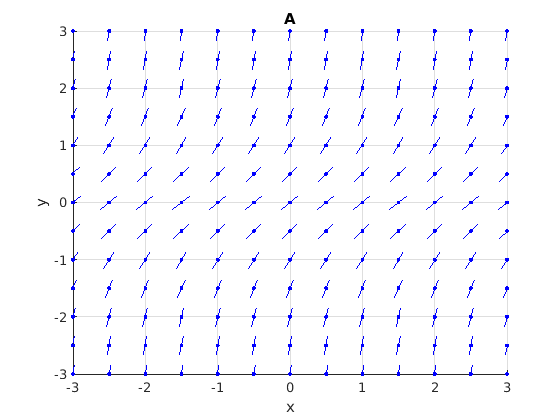
\includegraphics[width=8cm]{10_equ_diff/question2a}
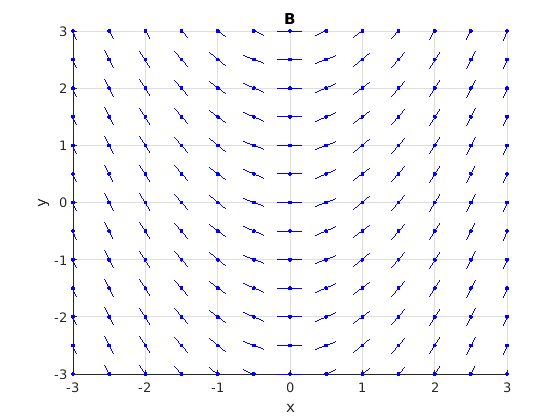
\includegraphics[width=8cm]{10_equ_diff/question2b}

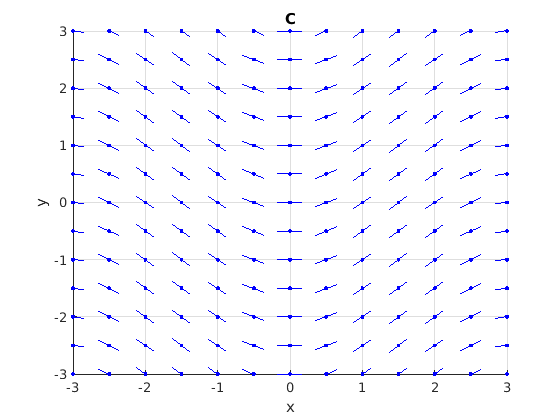
\includegraphics[width=8cm]{10_equ_diff/question2c}
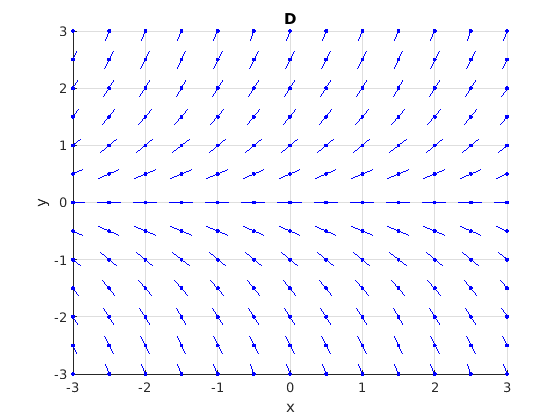
\includegraphics[width=8cm]{10_equ_diff/question2d}

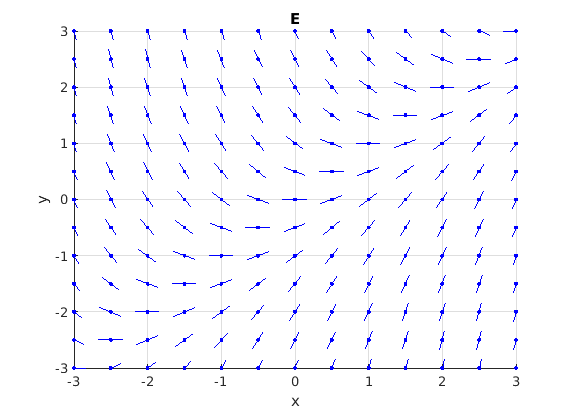
\includegraphics[width=8cm]{10_equ_diff/question2e}
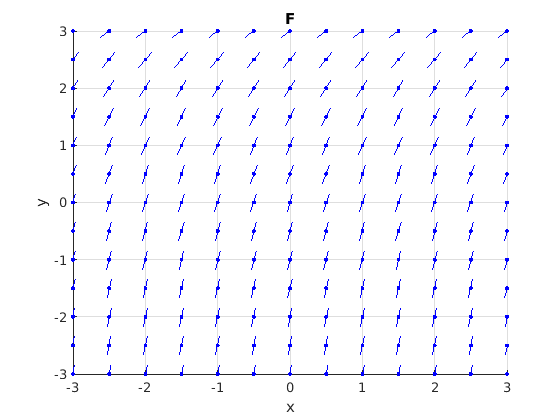
\includegraphics[width=8cm]{10_equ_diff/question2f}
\label{10Q45}
\end{question}

\begin{question}
Le champs de pentes de l'équation différentielle
\[
\dydx{y}{x} = (x-2)(x-y)
\]
est donné ci-dessous.
\MATHgraph{10_equ_diff/question3}{8cm}
\subQ{a} Tracez (de façon aussi précise que possible) le graphe de la
solution qui passe par le point $(0,0)$.\\
\subQ{b} Pour quelle valeur de $x$ la solution particulière qui passe
par le point $(0,0)$ a-t-elle un minimum local?  Un maximum local?
Justifiez vos réponses.\\ 
\subQ{c} Pour quelles régions du champs de pentes avons-nous que la pente est
positive.  Justifiez votre réponse en utilisant seulement
l'équation différentielle; sans utiliser le champ de pentes.
\label{10Q46}
\end{question}

\begin{question}
Considérons l'équation différentielle  $y' = -y/x$.\\
\subQ{a} Dessinez le champ de pentes de cet équation différentielle.\\
\subQ{b} Dessinez sur la même figure que celle pour votre champ de
pentes plusieurs solutions de cette équation différentielle.\\ 
\subQ{c} Trouvez la solution générale de l'équation différentielle.\\
\subQ{d} Que ce passe-t-il lorsque $x = 0$?
\label{10Q47}
\end{question}

\subsection{Applications}

\begin{question}[\eng]
En chimie, une {\bfseries équation de
  réaction-diffusion}\index{Équation de réaction diffusion}  est une
équation différentielle qui décrit la concentration d'un produit
chimique sous l'effet d'une réaction chimique et de la diffusion.  Un
exemple simple d'une telle équation est
\[
\dydx{C}{t} = \beta(\gamma-C) + \frac{C}{2+C}
\]
où le terme $\beta(\gamma-C)$ représente la diffusion et le terme
$\displaystyle \frac{C}{2+C}$ représente la réaction chimique.
les unités de la constante $\beta$ sont les m$^{-1}$ et les unités de la
constante $\gamma$ sont les mol/l.  Si $\beta=1$ et $\gamma=5$, trouvez les
points d'équilibre et déterminez leur stabilité.
\label{10Q48}
\end{question}

\begin{question}[\life]
L'équation différentielle suivante décrit la concentration $C(t)$ d'un
produit chimique au temps $t$ dans une cellule.
\begin{equation}\label{reactdiff}
\dydx{C}{t} = \beta(\Gamma-C) + 0.5\,C \ .
\end{equation}
Le terme $0.5 C$ représente la réaction en réponse à un facteur externe (la
cellule fabrique le produit chimique) et le terme $\beta(\Gamma -C)$
représente la diffusion au travers de la membrane de la cellule.  C'est un
exemple d'une
{\bfseries équation de réaction diffusion}\index{Équation de réaction
  diffusion}.

Répondez aux questions suivantes pour $\beta = 1.0$ min$^{-1}$ et
$\Gamma = 5.0$ mol/l.

\subQ{a} Quelles sont les points d'équilibre?

\subQ{b} Utilisez le théorème sur la stabilité des points d'équilibre pour
déterminez la stabilité des points d'équilibre que vous avez trouvés en
(a).

\subQ{c} Tracez le portrait de phases pour cette équation différentielle.

\subQ{d} Dessinez un champ de pentes et tracez quelques solutions.

\subQ{e} Quelles seraient les points d'équilibre s'il n'y avait pas le terme
de réaction (i.e. $0.5C$) dans l'équation différentielle ci-dessus.?
\label{10Q49}
\end{question}

\begin{question}[\life]
Un troupeau de gnous (de la famille des antilopes) habite une réserve
faunique.  La population initiale est de $1000$ gnous.  Après un an, la
population est de $1100$ gnous.  La population satisfait le modèle
logistique de croissance avec une capacité optimale pour le milieu de $1800$
gnous.  Combien de temps faut-il pour que la population atteigne $1500$
gnous?
\label{10Q50}
\end{question}

\begin{question}[\life]
Pour une certaine population, le nombre d'individus $N(t)$ par km$^2$
au temps $t$ satisfait
\begin{equation} \label{q5_edo}
\dydx{N}{t} = \frac{5\,N^2}{1+N^2} - 2\,N \ .
\end{equation}
\subQ{a} Quelles sont les points d'équilibre?

\subQ{b} Utilisez le théorème de stabilité des points d'équilibre pour
déterminer la stabilité des points d'équilibre que vous avez trouvés en
(a).

\subQ{c} Tracez le portrait de phases pour cette équation différentielle.

\subQ{d} Dessinez un champ de pentes et tracez quelques solutions.

\subQ{e} Déterminez le seuil de la population pour que celle-ci augmente?
\label{10Q51}
\end{question}

\begin{question}[\life]
Le modèle suivant est appelé le modèle de méta-population de Levins.
Pour étudier une population animale habitant un territoire, nous divisons le
territoire en petites sections.  Soit $p$ la fraction des sections qui sont
habitées et $d$ la fractions des sections qui sont détruites (e.g.\ par une
développeur immobilier).  Nous supposons que les sections détruites ne sont pas
habitées (et habitables).  La fraction $1-p$ est donc la fraction des
sections qui ne sont pas habitées et $1-p-d$ est la fraction des sections qui
ne sont pas habitées mais habitables.

La fraction de sections habitées est décrite par l'équation différentielle
\[
\dydx{p}{t} = c\,p(1-d-p)-m \,p
\]
où $m=1$ est le taux auquel les animaux d'une section habitée quittent cette
section et $c=2$ est le taux auquel les animaux s'installent dans une section
inhabitée et habitable.

Pour que le modèle soit consistant, il faut que $0\leq p \leq 1$ et
$0 \leq d \leq 1$.  De plus, il faut que $1 - p - d \geq 0$.
Il faut donc avoir en fait que $0 \leq p \leq 1 - d$.

\subQ{a} Trouvez les deux points d'équilibre de l'équation différentielle.
Un des points d'équilibre va dépende du paramètre $d$.  Pour quelles valeurs
de $d$ ce point d'équilibre a-t-il un sens biologique?

\subQ{b} Tracez le graphe de la fonction qui génère l'équation différentielle
et tracez le portrait de phases lorsque $d=1/4$ et $d=3/4.$

\subQ{c} Utilisez le test de la dérivée pour déterminer la stabilité des
deux points d'équilibres.  La stabilité va dépende de $d$.

\subQ{d} Est-ce que la population va survivre si $1/4$ des sections
(i.e.\ $d=1/4$) sont détruites?  Si $3/4$ des sections sont détruites?
\label{10Q52}
\end{question}

\begin{question}[\eng]
La concentration de sel dans un réservoir de $1000$ litres d'eau salée
est de $0.025$ kg par litre.  De l'eau salée dont la concentration de
sel est de $0.01$ kg par litre est ajoutée au réservoir à raison de
$10$ litres par minute.  De plus, $10$ litres d'eau salée par minute
s'échappe du réservoir.  Si le contenue du réservoir
est bien mélangé, combien de temps s'écoule-t-il avant que d'atteindre
une concentration de $0.02$ kg de sel par litre?
\label{10Q53}
\end{question}

\begin{question}[\eng]
Un réservoir contient $1000$ litres d'eau pure.  Une saumure contenant
$0.1$ kg de sel par litre d'eau est versée dans le réservoir au taux
de $5$ litres par minute.  Une saumure contenant $0.05$ kg de sel par
litre est aussi versée dans le réservoir au taux de $15$ litres par
minute.  En supposant que le contenu du réservoir est toujours bien
mélangé et que le réservoir perd $20$ litres par minutes, quelle est
la quantité de sel dans le réservoir après $t$ minutes?  quelle est la
concentration de sel dans le réservoir après $t$ minutes?
\label{10Q54}
\end{question}

\begin{question}[\life]
Considérons l'équation différentielle $\displaystyle \dydx{x}{t} = a x - x^2$
où $a$ est un paramètre.

\subQ{a} Trouvez les points d'équilibre de cette équation différentielle.  Un
des points d'équilibre devrait dépendre de $a$.

\subQ{b} Dans un même système de coordonnées, tracez le graphe de chacun des
points d'équilibre en fonction de $a$ pour $a$ au voisinage de l'origine.
Utilisez une ligne pleine pour les points d'équilibre stables et une ligne
hachurée pour les points d'équilibre instables.

\subQ{c} Que ce passe-t-il au voisinage de l'origine?  Ce genre de phénomène
est appelé {\em bifurcation}.  Dans le cas présent, nous parlons de
{\em bifurcation transcritique}.
\label{10Q55}
\end{question}

\begin{question}[\life]
Considérons l'équation logistique
\begin{equation}\label{ass_logistic}
\dydx{b}{t} = b(1-b) - hb
\end{equation}
pour une population animale où $h$ est la fraction de la population qui a été
récolté.

\subQ{a} Trouvez les points d'équilibre de (\ref{ass_logistic}).  Un des
points d'équilibre va dépendre de $h$.

\subQ{b} Dans un même système de coordonnées, tracez le graphe de chacun des
points d'équilibre en fonction de $h$ pour $0\leq h \leq 2$.  Utilisez une
ligne pleine pour les points d'équilibre stable et une ligne hachurée pour
les point d'équilibre instable.  Même s'ils n'ont pas de sens biologique,
inclure les valeurs négative des points d'équilibre.

\subQ{c} Quelle type de bifurcation obtenez-vous?
\label{10Q56}
\end{question}

\subsection{Méthode d'Euler}

\begin{question}[\theory]
Considérons l'équation différentielle $y'(x)=f(x)$ avec $y(0) = 0$.
Expliquez pourquoi l'approximation de $y(x)$ donnée par la méthode
d'Euler correspond à une somme de Reimann à droite associée a
l'intégrale $\displaystyle \int_0^x f(t) \dx{t} $.
\label{10Q57}
\end{question}

\begin{question}[\eng]
\subQ{a} Utiliser la méthode d'Euler pour trouver une approximation de
la solution $y(t)$ de
\[
\frac{\text{d}y}{\text{d}t} = 1/t
\]
à $t=2$.  Commencer à $(t,y) = (1,0)$ et utiliser $10$
sous-intervalles. \\
\subQ{b} Trouver la valeur exacte de $y(t)$ \`a $t = 2$.\\
\subQ{c} Est-ce que votre approximation de $y(t)$ à $t=2$ est plus
petite ou plus grande que la valeur exacte à $t=2$.  Utiliser le champ
de pentes (i.e. la courbure de la solution) pour expliquer la différence.
\label{10Q58}
\end{question}

\begin{question}[\eng]
Utilisez la méthode d'Euler avec $10$ sous-intervalles pour résoudre
numériquement l'équation différentielle
\begin{align*}
y' &= \frac{y + t}{t} \quad , \quad 1 \leq t \leq 2 \\
y(1) &= 0
\end{align*}
Est-ce que les valeurs données par la méthodes d'Euler sont des
surestimations ou des sous-estimations de la solution $y$?
\label{10Q59}
\end{question}

\begin{question}[\eng]
\subQ{a} Utilisez la méthode d'Euler avec $n=10$ sous-intervalles pour
trouver une approximation de $y(1)$ où $y$ est la solution de l'équation
différentielle $\displaystyle y'=\frac{3x^2}{2y}$ avec la condition
initiale $y(0)=1$.

\subQ{b} Trouvez la solution exacte de l'équation différentielle
$y'=\frac{3x^2}{2y}$ avec $y(0)=1$.

\subQ{c} Quelle est l'erreur absolue et l'erreur relative de
l'approximation de $y(1)$ trouvée en (a)?
\label{10Q60}
\end{question}


%%% Local Variables: 
%%% mode: latex
%%% TeX-master: "notes"
%%% End: 
